\documentclass[]{book}
\usepackage{lmodern}
\usepackage{amssymb,amsmath}
\usepackage{ifxetex,ifluatex}
\usepackage{fixltx2e} % provides \textsubscript
\ifnum 0\ifxetex 1\fi\ifluatex 1\fi=0 % if pdftex
  \usepackage[T1]{fontenc}
  \usepackage[utf8]{inputenc}
\else % if luatex or xelatex
  \ifxetex
    \usepackage{mathspec}
  \else
    \usepackage{fontspec}
  \fi
  \defaultfontfeatures{Ligatures=TeX,Scale=MatchLowercase}
\fi
% use upquote if available, for straight quotes in verbatim environments
\IfFileExists{upquote.sty}{\usepackage{upquote}}{}
% use microtype if available
\IfFileExists{microtype.sty}{%
\usepackage{microtype}
\UseMicrotypeSet[protrusion]{basicmath} % disable protrusion for tt fonts
}{}
\usepackage{hyperref}
\hypersetup{unicode=true,
            pdftitle={Loss Data Analytics},
            pdfauthor={An open text authored by the Actuarial Community},
            pdfborder={0 0 0},
            breaklinks=true}
\urlstyle{same}  % don't use monospace font for urls
\usepackage{natbib}
\bibliographystyle{econPeriod}
\usepackage{color}
\usepackage{fancyvrb}
\newcommand{\VerbBar}{|}
\newcommand{\VERB}{\Verb[commandchars=\\\{\}]}
\DefineVerbatimEnvironment{Highlighting}{Verbatim}{commandchars=\\\{\}}
% Add ',fontsize=\small' for more characters per line
\usepackage{framed}
\definecolor{shadecolor}{RGB}{248,248,248}
\newenvironment{Shaded}{\begin{snugshade}}{\end{snugshade}}
\newcommand{\KeywordTok}[1]{\textcolor[rgb]{0.13,0.29,0.53}{\textbf{#1}}}
\newcommand{\DataTypeTok}[1]{\textcolor[rgb]{0.13,0.29,0.53}{#1}}
\newcommand{\DecValTok}[1]{\textcolor[rgb]{0.00,0.00,0.81}{#1}}
\newcommand{\BaseNTok}[1]{\textcolor[rgb]{0.00,0.00,0.81}{#1}}
\newcommand{\FloatTok}[1]{\textcolor[rgb]{0.00,0.00,0.81}{#1}}
\newcommand{\ConstantTok}[1]{\textcolor[rgb]{0.00,0.00,0.00}{#1}}
\newcommand{\CharTok}[1]{\textcolor[rgb]{0.31,0.60,0.02}{#1}}
\newcommand{\SpecialCharTok}[1]{\textcolor[rgb]{0.00,0.00,0.00}{#1}}
\newcommand{\StringTok}[1]{\textcolor[rgb]{0.31,0.60,0.02}{#1}}
\newcommand{\VerbatimStringTok}[1]{\textcolor[rgb]{0.31,0.60,0.02}{#1}}
\newcommand{\SpecialStringTok}[1]{\textcolor[rgb]{0.31,0.60,0.02}{#1}}
\newcommand{\ImportTok}[1]{#1}
\newcommand{\CommentTok}[1]{\textcolor[rgb]{0.56,0.35,0.01}{\textit{#1}}}
\newcommand{\DocumentationTok}[1]{\textcolor[rgb]{0.56,0.35,0.01}{\textbf{\textit{#1}}}}
\newcommand{\AnnotationTok}[1]{\textcolor[rgb]{0.56,0.35,0.01}{\textbf{\textit{#1}}}}
\newcommand{\CommentVarTok}[1]{\textcolor[rgb]{0.56,0.35,0.01}{\textbf{\textit{#1}}}}
\newcommand{\OtherTok}[1]{\textcolor[rgb]{0.56,0.35,0.01}{#1}}
\newcommand{\FunctionTok}[1]{\textcolor[rgb]{0.00,0.00,0.00}{#1}}
\newcommand{\VariableTok}[1]{\textcolor[rgb]{0.00,0.00,0.00}{#1}}
\newcommand{\ControlFlowTok}[1]{\textcolor[rgb]{0.13,0.29,0.53}{\textbf{#1}}}
\newcommand{\OperatorTok}[1]{\textcolor[rgb]{0.81,0.36,0.00}{\textbf{#1}}}
\newcommand{\BuiltInTok}[1]{#1}
\newcommand{\ExtensionTok}[1]{#1}
\newcommand{\PreprocessorTok}[1]{\textcolor[rgb]{0.56,0.35,0.01}{\textit{#1}}}
\newcommand{\AttributeTok}[1]{\textcolor[rgb]{0.77,0.63,0.00}{#1}}
\newcommand{\RegionMarkerTok}[1]{#1}
\newcommand{\InformationTok}[1]{\textcolor[rgb]{0.56,0.35,0.01}{\textbf{\textit{#1}}}}
\newcommand{\WarningTok}[1]{\textcolor[rgb]{0.56,0.35,0.01}{\textbf{\textit{#1}}}}
\newcommand{\AlertTok}[1]{\textcolor[rgb]{0.94,0.16,0.16}{#1}}
\newcommand{\ErrorTok}[1]{\textcolor[rgb]{0.64,0.00,0.00}{\textbf{#1}}}
\newcommand{\NormalTok}[1]{#1}
\usepackage{longtable,booktabs}
\usepackage{graphicx,grffile}
\makeatletter
\def\maxwidth{\ifdim\Gin@nat@width>\linewidth\linewidth\else\Gin@nat@width\fi}
\def\maxheight{\ifdim\Gin@nat@height>\textheight\textheight\else\Gin@nat@height\fi}
\makeatother
% Scale images if necessary, so that they will not overflow the page
% margins by default, and it is still possible to overwrite the defaults
% using explicit options in \includegraphics[width, height, ...]{}
\setkeys{Gin}{width=\maxwidth,height=\maxheight,keepaspectratio}
\IfFileExists{parskip.sty}{%
\usepackage{parskip}
}{% else
\setlength{\parindent}{0pt}
\setlength{\parskip}{6pt plus 2pt minus 1pt}
}
\setlength{\emergencystretch}{3em}  % prevent overfull lines
\providecommand{\tightlist}{%
  \setlength{\itemsep}{0pt}\setlength{\parskip}{0pt}}
\setcounter{secnumdepth}{5}
% Redefines (sub)paragraphs to behave more like sections
\ifx\paragraph\undefined\else
\let\oldparagraph\paragraph
\renewcommand{\paragraph}[1]{\oldparagraph{#1}\mbox{}}
\fi
\ifx\subparagraph\undefined\else
\let\oldsubparagraph\subparagraph
\renewcommand{\subparagraph}[1]{\oldsubparagraph{#1}\mbox{}}
\fi

%%% Use protect on footnotes to avoid problems with footnotes in titles
\let\rmarkdownfootnote\footnote%
\def\footnote{\protect\rmarkdownfootnote}

%%% Change title format to be more compact
\usepackage{titling}

% Create subtitle command for use in maketitle
\providecommand{\subtitle}[1]{
  \posttitle{
    \begin{center}\large#1\end{center}
    }
}

\setlength{\droptitle}{-2em}

  \title{Loss Data Analytics}
    \pretitle{\vspace{\droptitle}\centering\huge}
  \posttitle{\par}
    \author{An open text authored by the Actuarial Community}
    \preauthor{\centering\large\emph}
  \postauthor{\par}
    \date{}
    \predate{}\postdate{}
  
\usepackage{booktabs}
\setcounter{secnumdepth}{2}

\begin{document}
\maketitle

{
\setcounter{tocdepth}{2}
\tableofcontents
}
\chapter*{Preface}\label{preface}
\addcontentsline{toc}{chapter}{Preface}

\emph{Date: 27 January 2020}

\subsubsection*{Book Description}\label{book-description}
\addcontentsline{toc}{subsubsection}{Book Description}

\textbf{Loss Data Analytics} is an interactive, online, freely available
text.

\begin{itemize}
\tightlist
\item
  The online version contains many interactive objects (quizzes,
  computer demonstrations, interactive graphs, video, and the like) to
  promote \emph{deeper learning}.
\item
  A subset of the book is available for \emph{offline reading} in pdf
  and EPUB formats.
\item
  The online text will be available in multiple languages to promote
  access to a \emph{worldwide audience}.
\end{itemize}

\subsubsection*{What will success look
like?}\label{what-will-success-look-like}
\addcontentsline{toc}{subsubsection}{What will success look like?}

The online text will be freely available to a worldwide audience. The
online version will contain many interactive objects (quizzes, computer
demonstrations, interactive graphs, video, and the like) to promote
deeper learning. Moreover, a subset of the book will be available in pdf
format for low-cost printing. The online text will be available in
multiple languages to promote access to a worldwide audience.

\subsubsection*{How will the text be
used?}\label{how-will-the-text-be-used}
\addcontentsline{toc}{subsubsection}{How will the text be used?}

This book will be useful in actuarial curricula worldwide. It will cover
the loss data learning objectives of the major actuarial organizations.
Thus, it will be suitable for classroom use at universities as well as
for use by independent learners seeking to pass professional actuarial
examinations. Moreover, the text will also be useful for the continuing
professional development of actuaries and other professionals in
insurance and related financial risk management industries.

\subsubsection*{Why is this good for the
profession?}\label{why-is-this-good-for-the-profession}
\addcontentsline{toc}{subsubsection}{Why is this good for the
profession?}

An online text is a type of open educational resource (OER). One
important benefit of an OER is that it equalizes access to knowledge,
thus permitting a broader community to learn about the actuarial
profession. Moreover, it has the capacity to engage viewers through
active learning that deepens the learning process, producing analysts
more capable of solid actuarial work.

Why is this good for students and teachers and others involved in the
learning process? Cost is often cited as an important factor for
students and teachers in textbook selection (see a recent post on the
\href{https://www.aei.org/publication/the-new-era-of-the-400-college-textbook-which-is-part-of-the-unsustainable-higher-education-bubble/}{\$400
textbook}). Students will also appreciate the ability to ``carry the
book around'' on their mobile devices.

\subsubsection*{Why loss data analytics?}\label{why-loss-data-analytics}
\addcontentsline{toc}{subsubsection}{Why loss data analytics?}

The intent is that this type of resource will eventually permeate
throughout the actuarial curriculum. Given the dramatic changes in the
way that actuaries treat data, loss data seems like a natural place to
start. The idea behind the name \emph{loss data analytics} is to
integrate classical loss data models from applied probability with
modern analytic tools. In particular, we recognize that big data
(including social media and usage based insurance) are here to stay and
that high speed computation is readily available.

\subsubsection*{Project Goal}\label{project-goal}
\addcontentsline{toc}{subsubsection}{Project Goal}

The project goal is to have the actuarial community author our textbooks
in a collaborative fashion. To get involved, please visit our
\href{https://sites.google.com/a/wisc.edu/loss-data-analytics/}{Open
Actuarial Textbooks Project Site}.

\section*{Acknowledgements}\label{acknowledgements}
\addcontentsline{toc}{section}{Acknowledgements}

Edward Frees acknowledges the John and Anne Oros Distinguished Chair for
Inspired Learning in Business which provided seed money to support the
project. Frees and his Wisconsin colleagues also acknowledge a Society
of Actuaries Center of Excellence Grant that provided funding to support
work in dependence modeling and health initiatives. Wisconsin also
provided an education innovation grant that provided partial support for
the many students who have worked on this project.

We acknowledge the Society of Actuaries for permission to use problems
from their examinations.

We thank Rob Hyndman, Monash University, for allowing us to use his
excellent style files to produce the online version of the book.

We thank Yihui Xie and his colleagues at
\href{https://www.rstudio.com/}{Rstudio} for the
\href{https://bookdown.org/yihui/bookdown/}{R bookdown} package that
allows us to produce this book.

We also wish to acknowledge the support and sponsorship of the
\href{http://www.blackactuaries.org/}{International Association of Black
Actuaries} in our joint efforts to provide actuarial educational content
to all.


\includegraphics[width=0.25000\textwidth]{Figures/IABA.png}

\section*{Contributors}\label{contributors}
\addcontentsline{toc}{section}{Contributors}

The project goal is to have the actuarial community author our textbooks
in a collaborative fashion. The following contributors have taken a
leadership role in developing \emph{Loss Data Analytics}.

\begin{itemize}
\item
  \textbf{Zeinab Amin} is the Director of the Actuarial Science Program
  and Associate Dean for Undergraduate Studies of the School of Sciences
  and Engineering at the American University in Cairo (AUC). Amin holds
  a PhD in Statistics and is an Associate of the Society of Actuaries.
  Amin is the recipient of the 2016 Excellence in Academic Service Award
  and the 2009 Excellence in Teaching Award from AUC. Amin has designed
  and taught a variety of statistics and actuarial science courses.
  Amin's current area of research includes quantitative risk assessment,
  reliability assessment, general statistical modelling, and Bayesian
  statistics.
\item
  \textbf{Katrien Antonio}, KU Leuven
\item
  \textbf{Jan Beirlant}, KU Leuven
\end{itemize}

\begin{itemize}
\tightlist
\item
  \textbf{Arthur Charpentier} is a professor in the Department of
  Mathematics at the Université du Québec á Montréal. Prior to that, he
  worked at a large general insurance company in Hong Kong, China, and
  the French Federation of Insurers in Paris, France. He received a MS
  on mathematical economics at Université Paris Dauphine and a MS in
  actuarial science at ENSAE (National School of Statistics) in Paris,
  and a PhD degree from KU Leuven, Belgium. His research interests
  include econometrics, applied probability and actuarial science. He
  has published several books (the most recent one on
  \emph{Computational Actuarial Science with R}, CRC) and papers on a
  variety of topics. He is a Fellow of the French Institute of
  Actuaries, and was in charge of the `Data Science for Actuaries'
  program from 2015 to 2018.
\end{itemize}

\begin{itemize}
\tightlist
\item
  \textbf{Curtis Gary Dean} is the Lincoln Financial Distinguished
  Professor of Actuarial Science at Ball State University. He is a
  Fellow of the Casualty Actuarial Society and a CFA charterholder. He
  has extensive practical experience as an actuary at American States
  Insurance, SAFECO, and Travelers. He has served the CAS and actuarial
  profession as chair of the Examination Committee, first
  editor-in-chief for \emph{Variance: Advancing the Science of Risk},
  and as a member of the Board of Directors and the Executive Council.
  He contributed a chapter to \emph{Predictive Modeling Applications in
  Actuarial Science} published by Cambridge University Press.
\end{itemize}

\begin{itemize}
\tightlist
\item
  \textbf{Edward W. (Jed) Frees} is an emeritus professor, formerly the
  Hickman-Larson Chair of Actuarial Science at the University of
  Wisconsin-Madison. He is a Fellow of both the Society of Actuaries and
  the American Statistical Association. He has published extensively (a
  four-time winner of the Halmstad and Prize for best paper published in
  the actuarial literature) and has written three books. He also is a
  co-editor of the two-volume series \emph{Predictive Modeling
  Applications in Actuarial Science} published by Cambridge University
  Press.
\end{itemize}

\begin{itemize}
\tightlist
\item
  \textbf{Guojun Gan} is an assistant professor in the Department of
  Mathematics at the University of Connecticut, where he has been since
  August 2014. Prior to that, he worked at a large life insurance
  company in Toronto, Canada for six years. He received a BS degree from
  Jilin University, Changchun, China, in 2001 and MS and PhD degrees
  from York University, Toronto, Canada, in 2003 and 2007, respectively.
  His research interests include data mining and actuarial science. He
  has published several books and papers on a variety of topics,
  including data clustering, variable annuity, mathematical finance,
  applied statistics, and VBA programming.
\end{itemize}

\begin{itemize}
\tightlist
\item
  \textbf{Lisa Gao} is a PhD candidate in the Risk and Insurance
  department at the University of Wisconsin-Madison. She holds a BMath
  in Actuarial Science and Statistics from the University of Waterloo
  and is an Associate of the Society of Actuaries.
\end{itemize}

\begin{itemize}
\tightlist
\item
  \textbf{José Garrido}, Concordia University
\end{itemize}

\begin{itemize}
\tightlist
\item
  \textbf{Lei (Larry) Hua} is an Associate Professor of Actuarial
  Science at Northern Illinois University. He earned a PhD degree in
  Statistics from the University of British Columbia. He is an Associate
  of the Society of Actuaries. His research work focuses on multivariate
  dependence modeling for non-Gaussian phenomena and innovative
  applications for financial and insurance industries.
\end{itemize}

\begin{itemize}
\tightlist
\item
  \textbf{Noriszura Ismail} is a Professor and Head of Actuarial Science
  Program, Universiti Kebangsaan Malaysia (UKM). She specializes in Risk
  Modelling and Applied Statistics. She obtained her BSc and MSc
  (Actuarial Science) in 1991 and 1993 from University of Iowa, and her
  PhD (Statistics) in 2007 from UKM. She also passed several papers from
  Society of Actuaries in 1994. She has received several research grants
  from Ministry of Higher Education Malaysia (MOHE) and UKM, totaling
  about MYR1.8 million. She has successfully supervised and
  co-supervised several PhD students (13 completed and 11 on-going). She
  currently has about 180 publications, consisting of 88 journals and 95
  proceedings.
\end{itemize}

\begin{itemize}
\tightlist
\item
  \textbf{Joseph H.T. Kim}, Ph.D., FSA, CERA, is Associate Professor of
  Applied Statistics at Yonsei University, Seoul, Korea. He holds a
  Ph.D.~degree in Actuarial Science from the University of Waterloo, at
  which he taught as Assistant Professor. He also worked in the life
  insurance industry. He has published papers in \emph{Insurance
  Mathematics and Economics}, \emph{Journal of Risk and Insurance},
  \emph{Journal of Banking and Finance}, \emph{ASTIN Bulletin}, and
  \emph{North American Actuarial Journal}, among others.
\end{itemize}

\begin{itemize}
\item
  \textbf{Nii-Armah Okine} is a dissertator at the business school of
  University of Wisconsin-Madison with a major in actuarial science. He
  obtained his master's degree in Actuarial science from Illinois State
  University. His research interests includes micro-level reserving,
  joint longitudinal-survival modeling, dependence modelling, micro
  insurance and machine learning.
\item
  \textbf{Margie Rosenberg} - University of Wisconsin
\end{itemize}

\begin{itemize}
\tightlist
\item
  \textbf{Emine Selin Sarıdaş} is a doctoral candidate in the Statistics
  department of Mimar Sinan University. She holds a bachelor degree in
  Actuarial Science with a minor in Economics and a master degree in
  Actuarial Science from Hacettepe University. Her research interest
  includes dependence modeling, regression, loss models and life
  contingencies.
\end{itemize}

\begin{itemize}
\tightlist
\item
  \textbf{Peng Shi} is an associate professor in the Risk and Insurance
  Department at the Wisconsin School of Business. He is also the Charles
  \& Laura Albright Professor in Business and Finance. Professor Shi is
  an Associate of the Casualty Actuarial Society (ACAS) and a Fellow of
  the Society of Actuaries (FSA). He received a Ph.D.~in actuarial
  science from the University of Wisconsin-Madison. His research
  interests are problems at the intersection of insurance and
  statistics. He has won several research awards, including the Charles
  A. Hachemeister Prize, the Ronald Bornhuetter Loss Reserve Prize, and
  the American Risk and Insurance Association Prize.
\end{itemize}

\begin{itemize}
\tightlist
\item
  \textbf{Nariankadu D. Shyamalkumar (Shyamal)} is an associate
  professor in the Department of Statistics and Actuarial Science at The
  University of Iowa. He is an Associate of the Society of Actuaries,
  and has volunteered in various elected and non-elected roles within
  the SoA. Having a broad theoretical interest as well as interest in
  computing, he has published in prominent actuarial, computer science,
  probability theory, and statistical journals. Moreover, he has worked
  in the financial industry, and since then served as an independent
  consultant to the insurance industry. He has experience educating
  actuaries in both Mexico and the US, serving in the roles of directing
  an undergraduate program, and as a graduate adviser for both masters
  and doctoral students.
\end{itemize}

\begin{itemize}
\tightlist
\item
  \textbf{Jianxi Su} is an Assistant Professor at the Department of
  Statistics at Purdue University. He is the Associate Director of
  Purdue's Actuarial Science. Prior to joining Purdue in 2016, he
  completed the PhD at York University (2012-2015). He obtained the
  Fellow of the Society of Actuaries (FSA) in 2017. His research
  expertise are in dependence modelling, risk management, and pricing.
  During the PhD candidature, Jianxi also worked as a research associate
  at the Model Validation and ORSA Implementation team of Sun Life
  Financial (Toronto office).
\end{itemize}

\begin{itemize}
\tightlist
\item
  \textbf{Tim Verdonck} is associate professor at the University of
  Antwerp. He has a degree in Mathematics and a PhD in Science:
  Mathematics, obtained at the University of Antwerp. During his PhD he
  successfully took the Master in Insurance and the Master in Financial
  and Actuarial Engineering, both at KU Leuven. His research focuses on
  the adaptation and application of robust statistical methods for
  insurance and finance data.
\end{itemize}

\begin{itemize}
\tightlist
\item
  \textbf{Krupa Viswanathan} is an Associate Professor in the Risk,
  Insurance and Healthcare Management Department in the Fox School of
  Business, Temple University. She is an Associate of the Society of
  Actuaries. She teaches courses in Actuarial Science and Risk
  Management at the undergraduate and graduate levels. Her research
  interests include corporate governance of insurance companies, capital
  management, and sentiment analysis. She received her Ph.D.~from The
  Wharton School of the University of Pennsylvania.
\end{itemize}

\section*{Reviewers}\label{reviewers}
\addcontentsline{toc}{section}{Reviewers}

Our goal is to have the actuarial community author our textbooks in a
collaborative fashion. Part of the writing process involves many
reviewers who generously donated their time to help make this book
better. They are:

\begin{itemize}
\tightlist
\item
  Yair Babab
\item
  Chunsheng Ban, Ohio State University
\item
  Vytaras Brazauskas, University of Wisconsin - Milwaukee
\item
  Chun Yong Chew, Universiti Tunku Abdul Rahman (UTAR)
\item
  Eren Dodd, University of Southampton
\item
  Gordon Enderle, University of Wisconsin - Madison
\item
  Rob Erhardt, Wake Forest University
\item
  Runhun Feng, University of Illinois
\item
  Liang (Jason) Hong, Robert Morris University
\item
  Fei Huang, Australian National University
\item
  Hirokazu (Iwahiro) Iwasawa
\item
  Himchan Jeong, University of Connecticut
\item
  Min Ji, Towson University
\item
  Paul Herbert Johnson, University of Wisconsin - Madison
\item
  Samuel Kolins, Lebonan Valley College
\item
  Andrew Kwon-Nakamura, Zurich North America
\item
  Ambrose Lo, University of Iowa
\item
  Mark Maxwell, University of Texas at Austin
\item
  Tatjana Miljkovic, Miami University
\item
  Bell Ouelega, American University in Cairo
\item
  Zhiyu (Frank) Quan, University of Connecticut
\item
  Jiandong Ren, Western University
\item
  Rajesh V. Sahasrabuddhe, Oliver Wyman
\item
  Ranee Thiagarajah, Illinois State University
\item
  Ping Wang, Saint Johns University
\item
  Chengguo Weng, University of Waterloo
\item
  Toby White, Drake University
\item
  Michelle Xia, Northern Illinois University
\item
  Di (Cindy) Xu, University of Nebraska - Lincoln
\item
  Lina Xu, Columbia University
\item
  Lu Yang, University of Amsterdam
\item
  Jorge Yslas, University of Copenhagen
\item
  Jeffrey Zheng, Temple University
\item
  Hongjuan Zhou, Arizona State University
\end{itemize}

\section*{For our Readers}\label{for-our-readers}
\addcontentsline{toc}{section}{For our Readers}

We hope that you find this book worthwhile and even enjoyable. For your
convenience, at our \href{https://openacttexts.github.io/}{Github
Landing site} (\url{https://openacttexts.github.io/}), you will find
links to the book that you can (freely) download for offline reading,
including a pdf version (for Adobe Acrobat) and an EPUB version suitable
for mobile devices.
\href{https://github.com/OpenActTexts/Loss-Data-Analytics/tree/master/Data}{Data}
for running our examples are available at the same site.

In developing this book, we are emphasizing the
\href{https://openacttexts.github.io/Loss-Data-Analytics/index.html}{online
version} that has lots of great features such as a glossary, code and
solutions to examples that you can be revealed interactively. For
example, you will find that the statistical code is hidden and can only
be seen by clicking on terms such as

We hide the code because we don't want to insist that you use the
\texttt{R} statistical software (although we like it). Still, we
encourage you to try some statistical code as you read the book -- we
have opted to make it easy to learn \texttt{R} as you go. We have even
set up a separate \href{https://openacttexts.github.io/LDARcode}{R Code
for Loss Data Analytics} site to explain more of the details of the
code.

Freely available, interactive textbooks represent a new venture in
actuarial education and we need your input. Although a lot of effort has
gone into the development, we expect hiccoughs. Please let your
instructor know about opportunities for improvement, write us through
our project site, or contact chapter contributors directly with
suggested improvements.

\chapter{Loss Reserving}\label{C:LossReserves}

\emph{Chapter Preview.} This chapter introduces loss reserving (also
known as claims reserving) for property and casualty (P\&C, or general,
non-life) insurance products. In particular, the chapter sketches some
basic, though essential, analytic tools to assess the reserves on a
portfolio of P\&C insurance products. First, Section \ref{S:motivation}
motivates the need for loss reserving, then Section \ref{S:Data} studies
the available data sources and introduces some formal notation to tackle
loss reserving as a prediction challenge. Next, Section
\ref{S:Chain-ladder} covers the chain-ladder method and Mack's
distribution-free chain-ladder model. Section \ref{S:GLMs} then develops
a fully stochastic approach to determine the outstanding reserve with
generalized linear models (GLMs), including the technique of
bootstrapping to obtain a predictive distribution of the outstanding
reserve via simulation.

\section{Motivation}\label{S:motivation}

Our starting point is the lifetime of a P\&C insurance claim. Figure
\ref{fig:tikz-run-off} pictures the development of such a claim over
time and identifies the events of interest:

\begin{figure}

{\centering 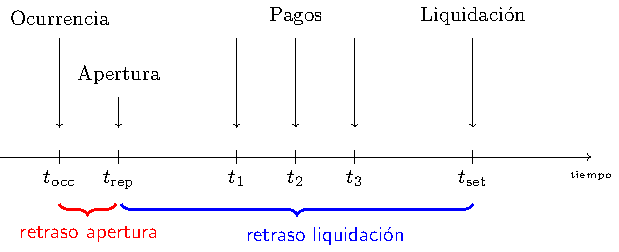
\includegraphics{LossDataAnalytics_files/figure-latex/tikz-run-off-1} 

}

\caption{Lifetime or run-off of a claim}\label{fig:tikz-run-off}
\end{figure}

The insured event or accident occurs at time \(t_{occ}\). This incident
is reported to the insurance company at time \(t_{rep}\), after some
delay. If the filed claim is accepted by the insurance company, payments
will follow to reimburse the financial loss of the policyholder. In this
example the insurance company compensates the incurred loss with loss
payments at times \(t_1\), \(t_2\) and \(t_3\). Eventually, the claim
settles or closes at time \(t_{set}\).

Often claims will not settle immediately due to the presence of delay in
the reporting of a claim, delay in the settlement process or both. The
reporting delay is the time that elapses between the occurrence of the
insured event and the reporting of this event to the insurance company.
The time between reporting and settlement of a claim is known as the
settlement delay. For example, it is very intuitive that a material
damage claim settles quicker than a bodily injury claim involving a
complex type of injury. Closed claims may also reopen due to new
developments, e.g.~an injury that requires extra treatment. Put
together, the development of a claim typically takes some time. The
presence of this delay in the run-off of a claim requires the insurer to
hold capital in order to settle these claims in the future.

\subsection{Closed, IBNR, and RBNS Claims}\label{S:claim-types}

Based on the status of the claim's run-off we distinguish three types of
claims in the books of an insurance company. A first type of claim is a
closed claim. For these claims the complete development has been
observed. With the red line in Figure \ref{fig:tikz-closed} indicating
the present moment, all events from the claim's development take place
before the present moment. Hence, these events are observed at the
present moment. For convenience, we will assume that a closed claim can
not reopen.

\begin{figure}

{\centering 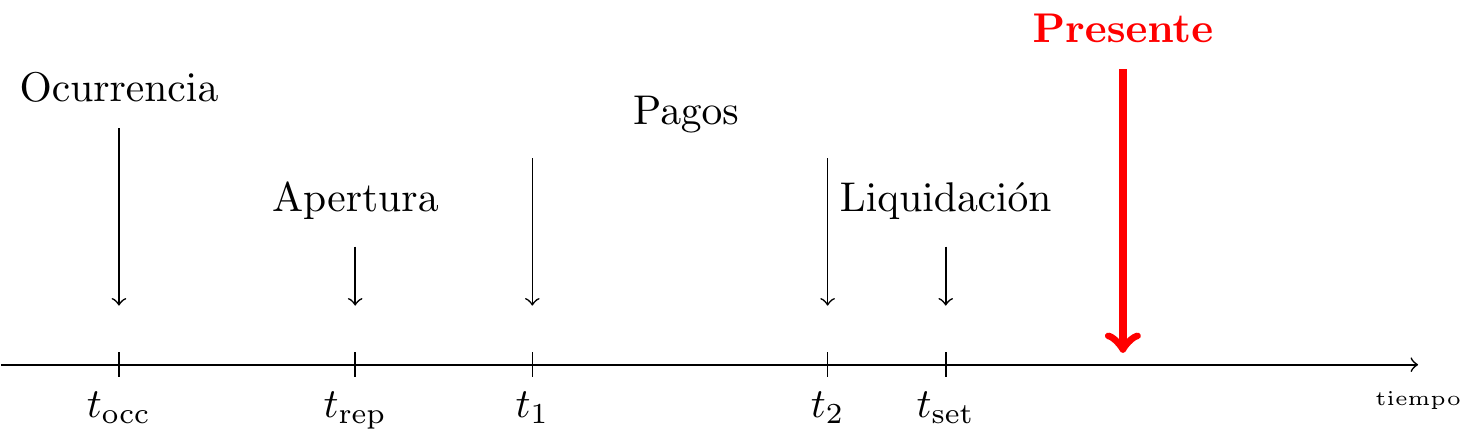
\includegraphics{LossDataAnalytics_files/figure-latex/tikz-closed-1} 

}

\caption{Lifetime of a closed claim}\label{fig:tikz-closed}
\end{figure}

An RBNS claim is one that has been \textbf{R}eported, \textbf{B}ut is
\textbf{N}ot fully \textbf{S}ettled at the present moment or the moment
of evaluation, that is, the moment when the reserves should be
calculated and booked by the insurer. Occurrence, reporting and possibly
some loss payments take place before the present moment, but the closing
of the claim happens in the future, beyond the present moment.

\begin{figure}

{\centering 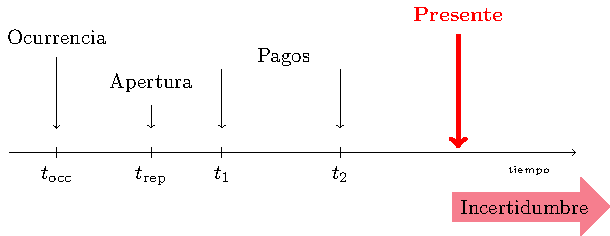
\includegraphics{LossDataAnalytics_files/figure-latex/tikz-RBNS-1} 

}

\caption{Lifetime of an RBNS claim}\label{fig:tikz-RBNS}
\end{figure}

An IBNR claim is one that has \textbf{I}ncurred in the past \textbf{B}ut
is \textbf{N}ot yet \textbf{R}eported. For such a claim the insured
event took place, but the insurance company is not yet aware of the
associated claim. This claim will be reported in the future and its
complete development (from reporting to settlement) takes place in the
future.

\begin{figure}

{\centering 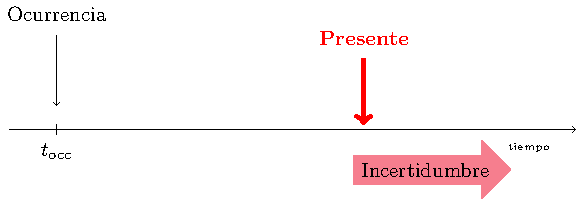
\includegraphics{LossDataAnalytics_files/figure-latex/tikz-IBNR-1} 

}

\caption{Lifetime of an IBNR claim}\label{fig:tikz-IBNR}
\end{figure}

Insurance companies will reserve capital to fulfill their future
liabilities with respect to both RBNS as well as IBNR claims. The future
development of such claims is uncertain and predictive modeling
techniques will be used to calculate appropriate reserves, from the
historical development data observed on similar claims.

\subsection{Why Reserving?}\label{why-reserving}

The inverted production cycle of the insurance market and the claim
dynamics pictured in Section \ref{S:claim-types} motivate the need for
reserving and the design of predictive modeling tools to estimate
reserves. In insurance, the premium income precedes the costs. An
insurer will charge a client a premium, before actually knowing how
costly the insurance policy or contract will become. In typical
manufacturing industry this is not the case and the manufacturer knows -
before selling a product - what the cost of producing this product was.
At a specified evaluation moment \(\tau\) the insurer will predict his
outstanding liabilities with respect to contracts sold in the past. This
is the claims reserve or loss reserve; it is the capital necessary to
settle open claims from past exposures. It is a very important element
on the balance sheet of the insurer, more specifically on the
liabilities side of this balance sheet.

\section{Loss Reserve Data}\label{S:Data}

\subsection{From Micro to Macro}\label{from-micro-to-macro}

We now shed light on the data available to estimate the outstanding
reserve for a portfolio of P\&C contracts. Insurance companies typically
register data on the development of an individual claim as sketched in
the timeline on the left hand side of Figure \ref{fig:tikz-micro-macro}.
We refer to data registered at this level as \textbf{granular or
micro-level} data. Typically, an actuary aggregates the information
registered on the individual development of claims across all claims in
a portfolio. This aggregation leads to data structured in a triangular
format as shown on the right hand side of Figure
\ref{fig:tikz-micro-macro}. Such data are called \textbf{aggregate or
macro-level} data because each cell in the triangle displays information
obtained by aggregating the development of multiple claims.

\begin{figure}

{\centering 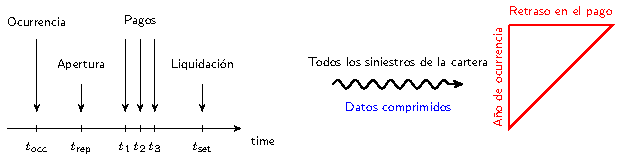
\includegraphics{LossDataAnalytics_files/figure-latex/tikz-micro-macro-1} 

}

\caption{From granular data to run-off triangle}\label{fig:tikz-micro-macro}
\end{figure}

The triangular display used in loss reserving is called a
\textbf{run-off or development} triangle. On the vertical axis the
triangle lists the accident or occurrence years during which a portfolio
is followed. The loss payments booked for a specific claim are connected
to the year during the which the insured event occurred. The horizontal
axis indicates the payment delay since occurrence of the insured event.

\subsection{Run-off Triangles}\label{run-off-triangles}

A first example of a run-off triangle with incremental payments is
displayed in Figure \ref{fig:tikz-triangle} (taken from
\citet{WuthrichMerz2008}, Table 2.2, also used in
\citet{WuthrichMerz2015}, Table 1.4). Accident years (or years of
occurrence) are shown on the vertical axis and run from 2004 up to 2013.
These refer to the year during which the insured event occurred. The
horizontal axis indicates the payment delay in years since occurrence of
the insured event. \emph{0 delay} is used for payments made in the year
of occurrence of the accident or insured event. \emph{One year} of delay
is used for payments made in the year after occurrence of the accident.

\begin{figure}

{\centering 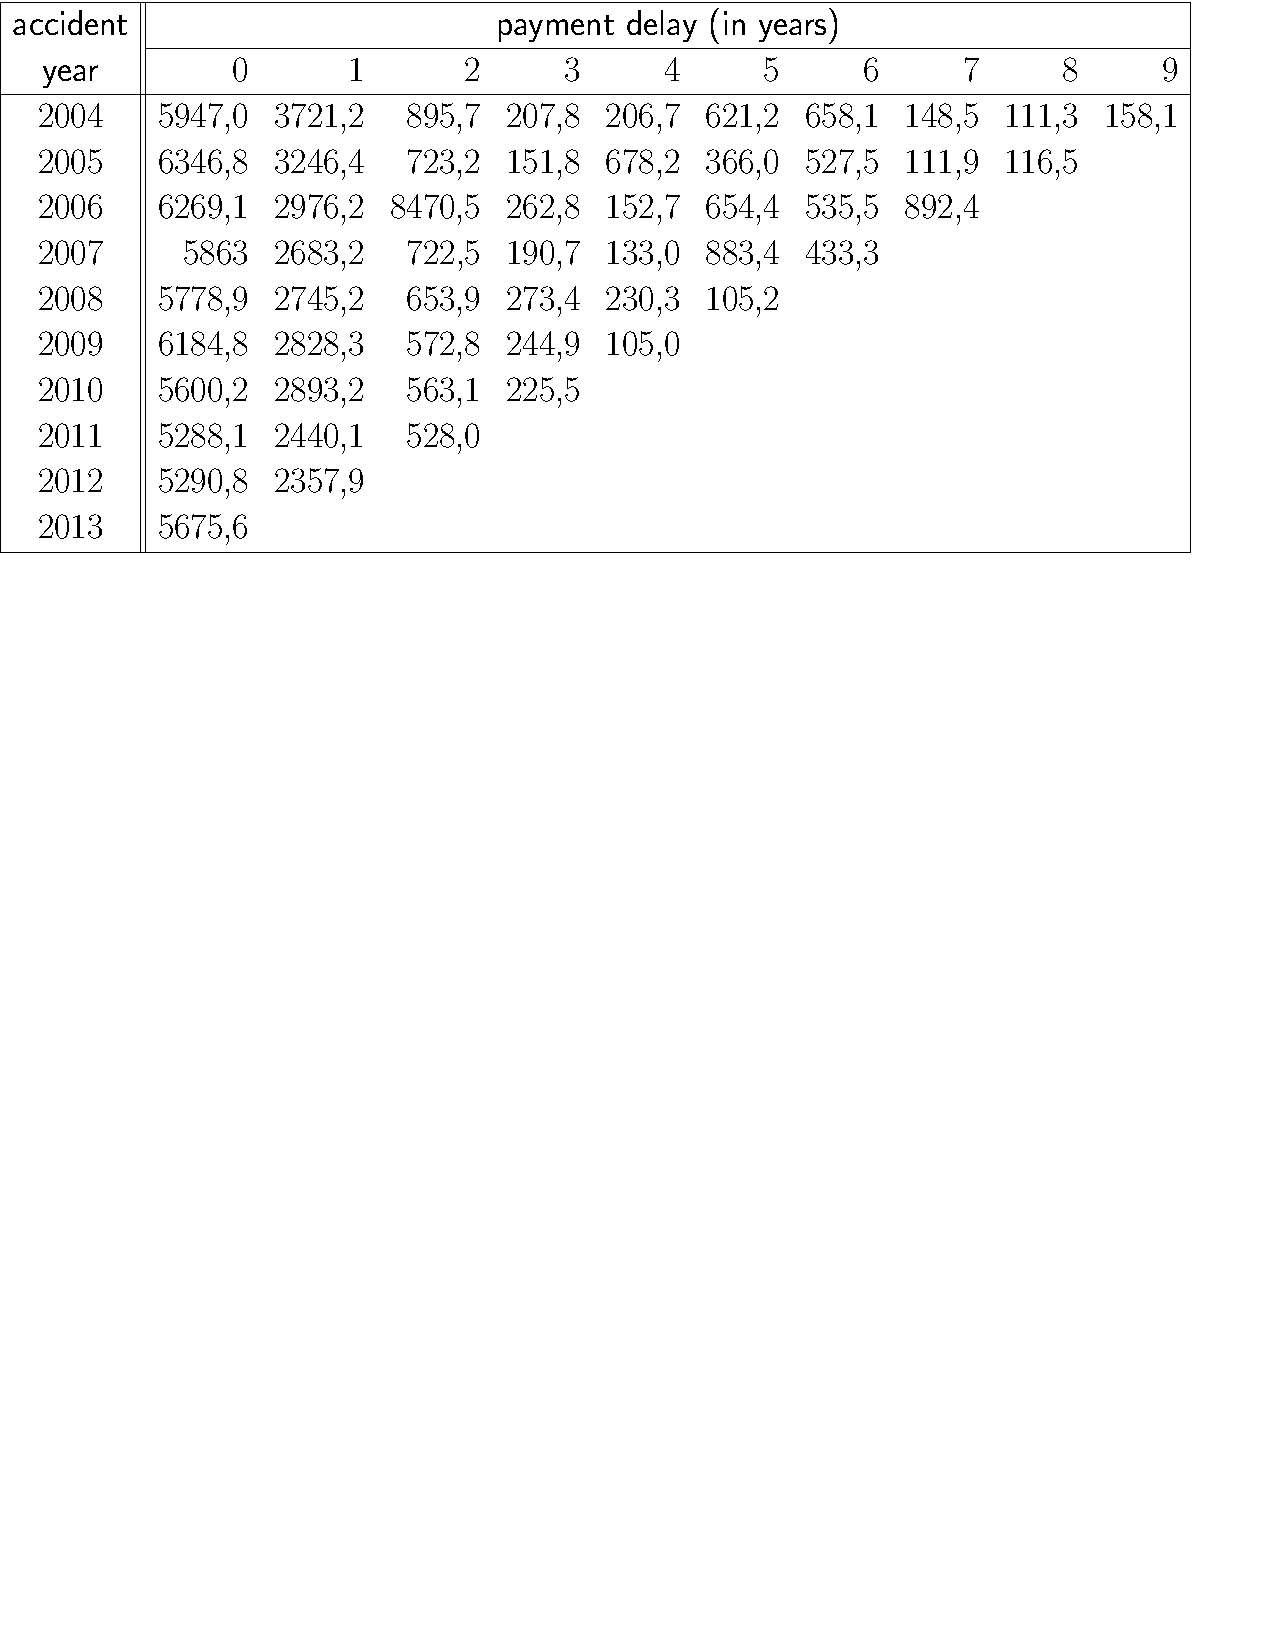
\includegraphics{LossDataAnalytics_files/figure-latex/tikz-triangle-1} 

}

\caption{A run-off triangle with incremental payment data. Source: @WuthrichMerz2008, Table 2.2.}\label{fig:tikz-triangle}
\end{figure}

For example, cell \((2004, 0)\) in the above triangle displays the
number \(5,947\), the total amount paid in the year 2004 for all claims
occurring in year 2004. Thus, it is the total amount paid with 0 years
of delay on all claims that occurred in the year 2004. Similarly, the
number in cell \((2012,1)\) displays the total \(2,357.9\) paid in the
year 2013 for all claims that occurred in year 2012.

\begin{figure}

{\centering 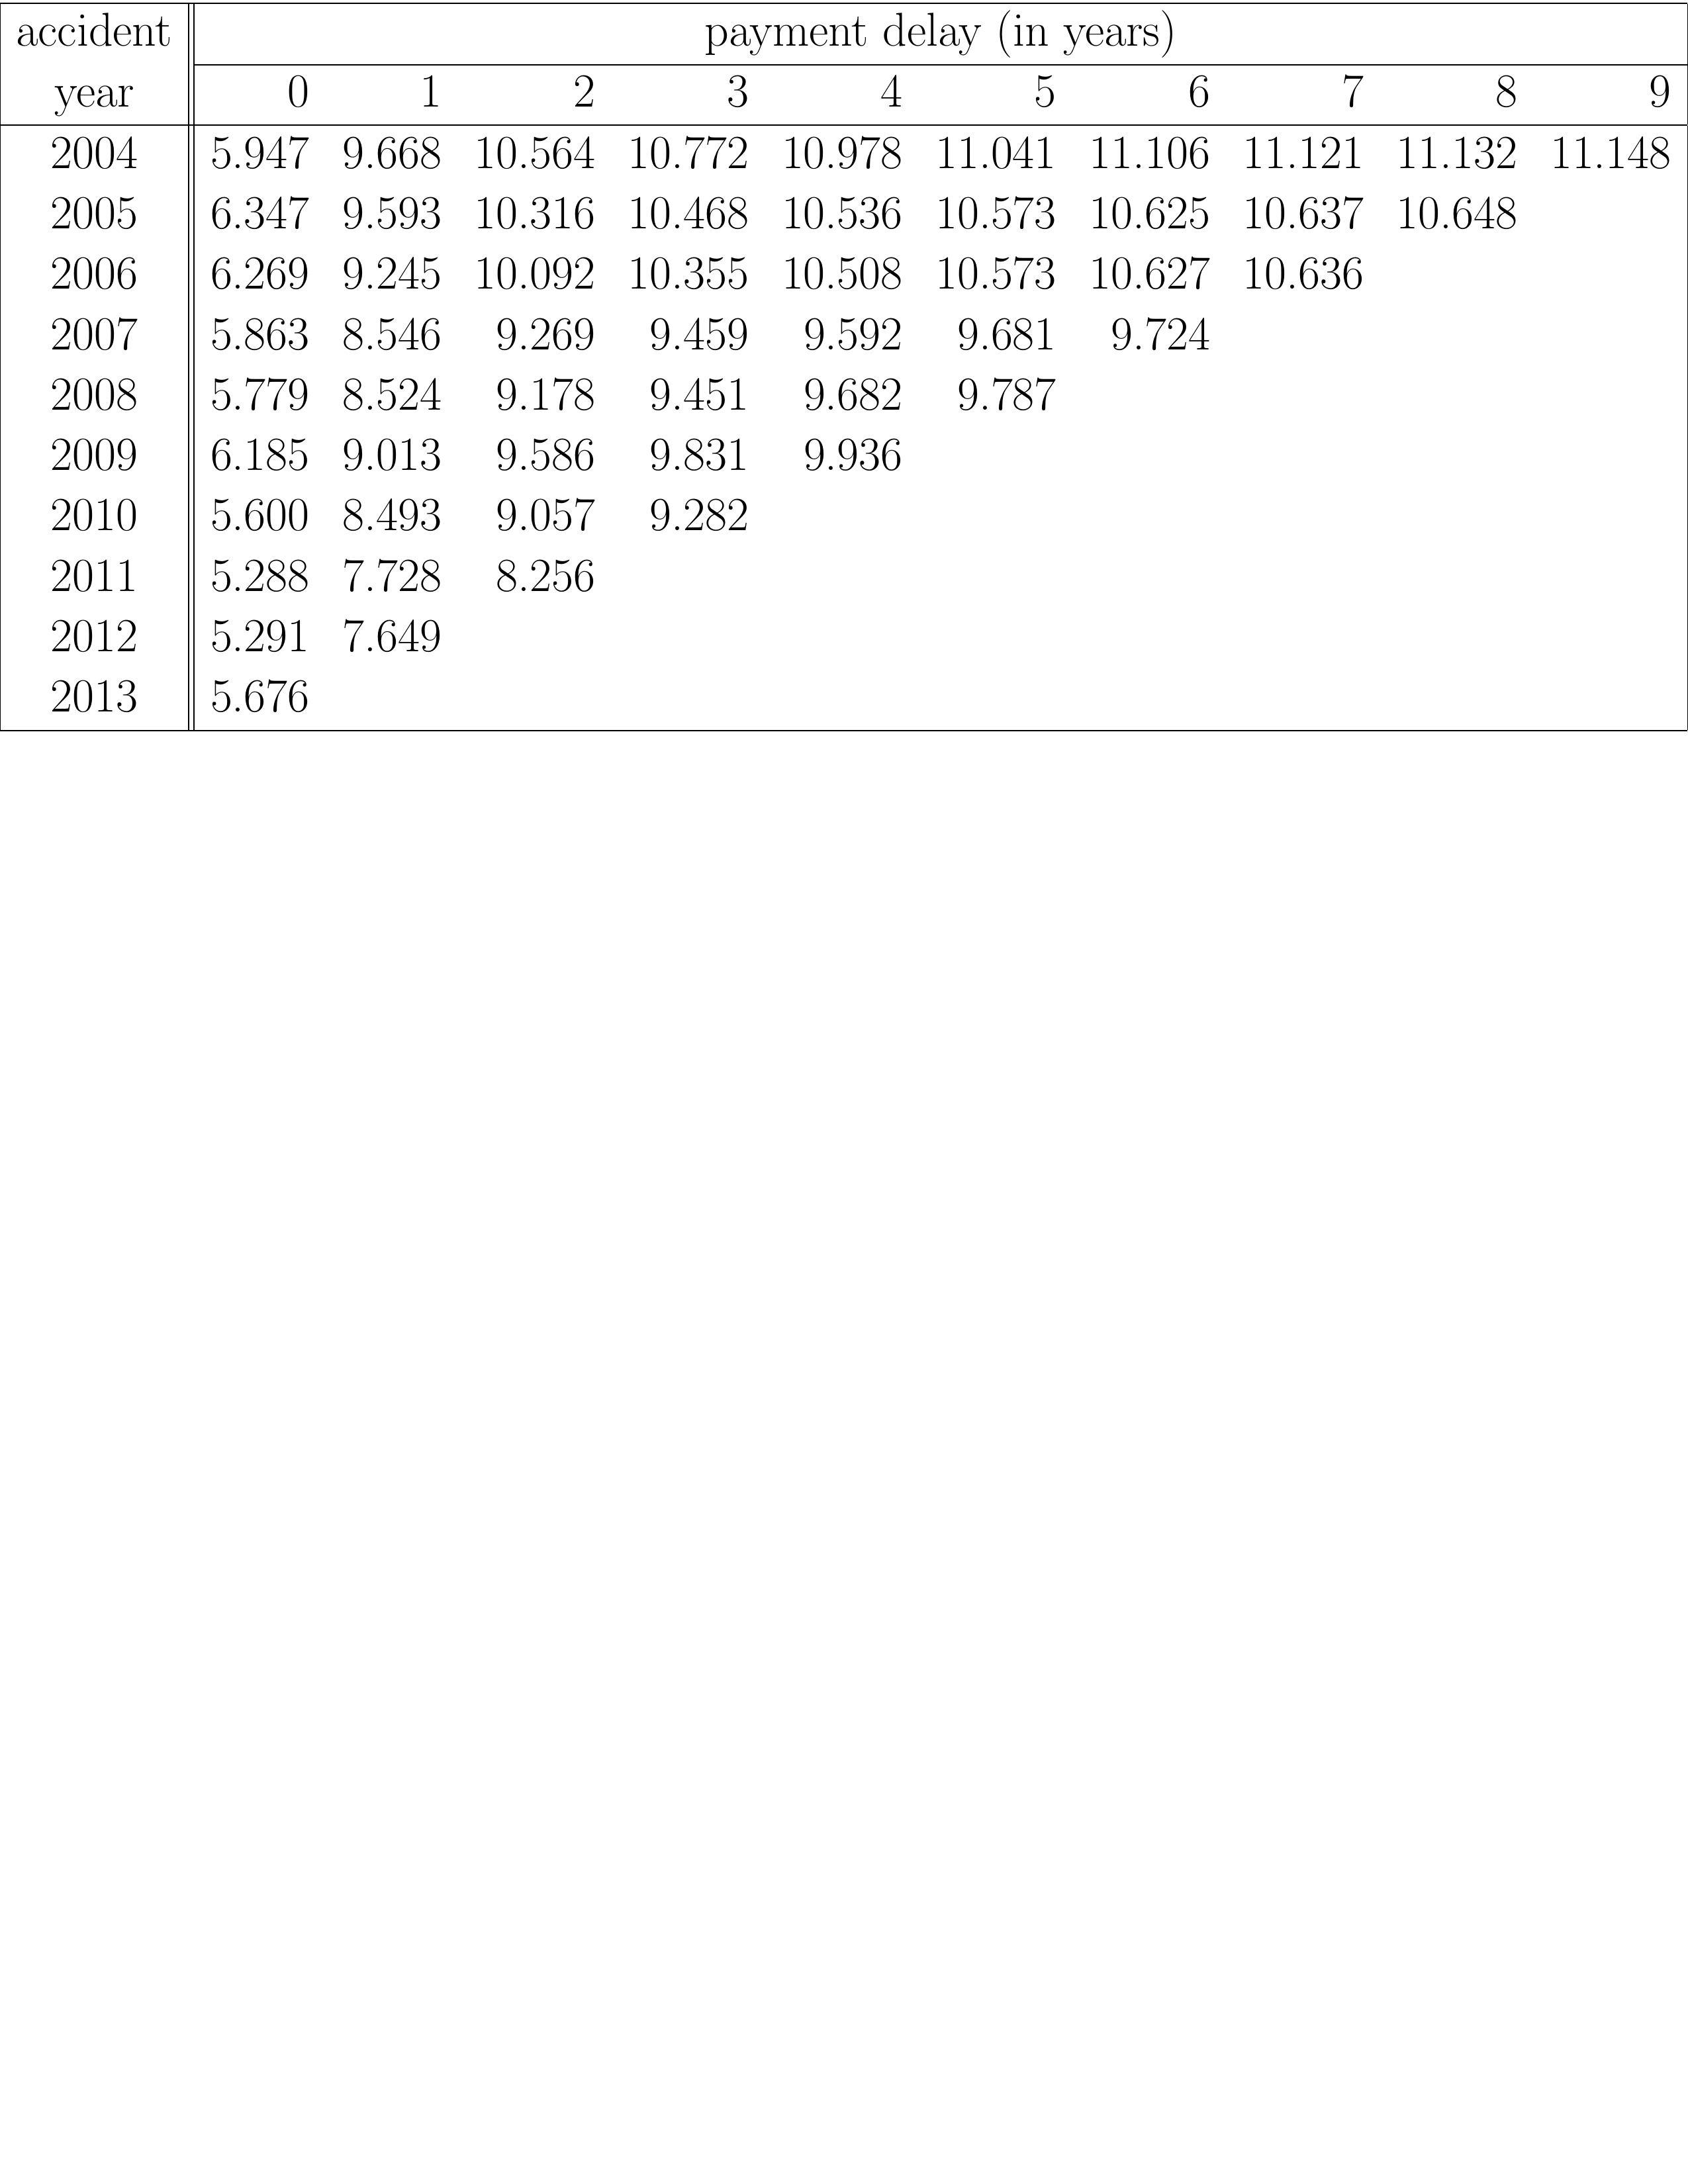
\includegraphics{LossDataAnalytics_files/figure-latex/tikz-cum-triangle-1} 

}

\caption{A run-off triangle with cumulative payment data. Source: @WuthrichMerz2008, Table 2.2.}\label{fig:tikz-cum-triangle}
\end{figure}

Whereas the triangle in Figure \ref{fig:tikz-triangle} displays
incremental payment data, the Figure \ref{fig:tikz-cum-triangle} shows
the same information in cumulative format. Now, cell \((2004,1)\)
displays the total claim amount paid \emph{up to} payment delay 1 for
all claims that occurred in year 2004. Therefore, it is the sum of the
amount paid in 2004 and the amount paid in 2005 on accidents that
occurred in 2004.

Different pieces of information can be stored in run-off triangles as
those shown in Figure \ref{fig:tikz-triangle} and Figure
\ref{fig:tikz-cum-triangle}. Depending on the kind of data stored, the
triangle will be used to estimate different quantities.

For example, in incremental format a cell may display:

\begin{itemize}
\tightlist
\item
  the claim payments, as motivated before
\item
  the number of claims that occurred in a specific year and were
  reported with a certain delay, when the goal is to estimate the number
  of IBNR claims
\item
  the change in incurred amounts, where incurred claim amounts are the
  sum of cumulative paid claims and the case estimates. The case
  estimate is the claims handler's expert estimate of the outstanding
  amount on a claim.
\end{itemize}

In cumulative format a cell may display:

\begin{itemize}
\tightlist
\item
  the cumulative paid amount, as motivated before
\item
  the total number of claims from an occurrence year, reported up to a
  certain delay
\item
  the incurred claim amounts.
\end{itemize}

Other sources of information are potentially available, e.g.~covariates
(like the type of claim), external information (like inflation, change
in regulation). Most claims reserving methods designed for run-off
triangles are rather based on a single source of information, although
recent contributions focus on the use of more detailed data for loss
reserving.

\subsection{Loss Reserve Notation}\label{loss-reserve-notation}

\subsubsection*{Run-off Triangles}\label{run-off-triangles-1}
\addcontentsline{toc}{subsubsection}{Run-off Triangles}

To formalize the displays shown in Figures \ref{fig:tikz-triangle} and
\ref{fig:tikz-cum-triangle}, we let \(i\) refer to the occurrence or
accident year, the year in which the insured event happened. In our
notation the first accident year considered in the portfolio is denoted
with 1 and the latest, most recent accident year is denoted with \(I\).
Then, \(j\) refers to the payment delay or development year, where a
delay equal to 0 corresponds to the accident year itself. Figure
\ref{fig:tikz-math-triangle} shows a triangle where the same number of
years is considered in both the vertical as well as the horizontal
direction, hence \(j\) runs from 0 up to \(J = I-1\).

\begin{figure}

{\centering 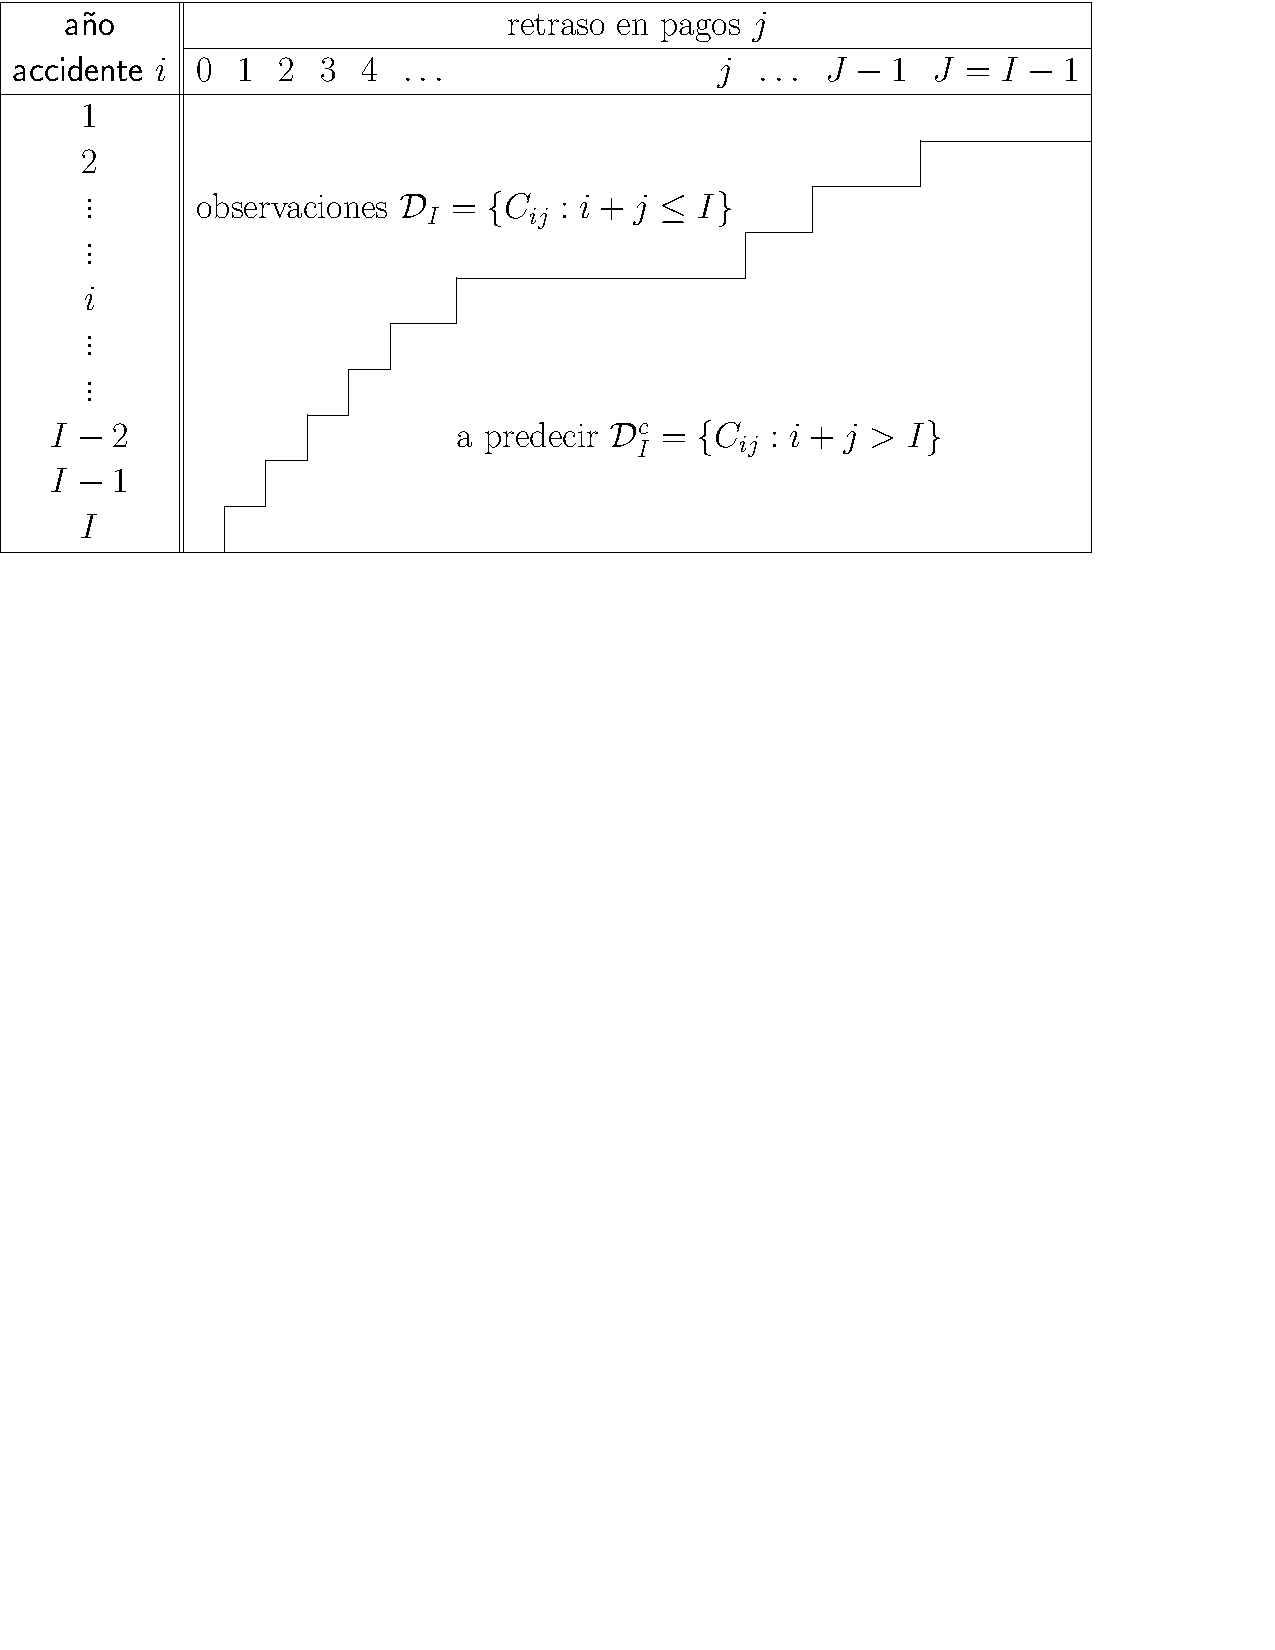
\includegraphics{LossDataAnalytics_files/figure-latex/tikz-math-triangle-1} 

}

\caption{Mathematical notation for a run-off triangle. Source: @WuthrichMerz2008}\label{fig:tikz-math-triangle}
\end{figure}

The random variable \(X_{ij}\) denotes the incremental claims paid in
development period \(j\) on claims from accident year \(i\). Thus,
\(X_{ij}\) is the total amount paid in development year \(j\) for all
claims that happened in occurrence year \(i\). These payments are
actually paid out in accounting or calendar year \(i+j\). Taking a
cumulative point of view, \(C_{ij}\) is the cumulative amount paid up
until (and including) development year \(j\) for accidents that occurred
in year \(i\). Ultimately, a total amount \(C_{iJ}\) is paid in the
final development year \(J\) for claims that occurred in accident year
\(i\). In this chapter time is expressed in years, though other time
units can be used as well, e.g.~semesters or quarters.

\subsubsection*{The Loss Reserve}\label{the-loss-reserve}
\addcontentsline{toc}{subsubsection}{The Loss Reserve}

At the evaluation moment \(\tau\), the data in the upper triangle have
been observed, whereas the lower triangle has to be predicted. Here, the
evaluation moment is the end of accident year \(I\) which implies that a
cell \((i,j)\) with \(i+j \leq I\) is observed, and a cell \((i,j)\)
with \(i+j > I\) belongs to the future and has to be predicted. Thus,
for a cumulative run-off triangle, the goal of a loss reserving method
is to predict \(C_{i,I-1}\), the ultimate claim amount for occurrence
year \(i\), corresponding to the final development period \(I-1\) in
Figure \ref{fig:tikz-cum-triangle}. We assume that - beyond this period
- no further payments will follow, although this assumption can be
relaxed.

Since \(C_{i,I-1}\) is cumulative, it includes both an observed part as
well as a part that has to be predicted. Therefore, the outstanding
liability or loss reserve for accident year \(i\) is

\begin{eqnarray*}
\mathcal{R}^{(0)}_{i} = \sum_{\ell=I-i+1}^{I-1} X_{i\ell} = C_{i,I}-C_{i,I-i}.
\end{eqnarray*}

We express the reserve either as a sum of incremental data, the
\(X_{i\ell}\), or as a difference between cumulative numbers. In the
latter case the outstanding amount is the ultimate cumulative amount
\(C_{i,I}\) minus the most recently observed cumulative amount
\(C_{i,I-i}\). Following \citet{WuthrichMerz2015}, the notation
\(\mathcal{R}^{(0)}_{i}\) refers to the reserve for occurrence year
\(i\) where \(i=1,\ldots,I\). The superscript \((0)\) refers to the
evaluation of the reserve at the present moment, say \(\tau = 0\). We
understand \(\tau = 0\) at the end of occurrence year \(I\), the most
recent calendar year for which data are observed and registered.

\subsection{R Code to Summarize Loss Reserve Data}\label{S:Rcode}

We use the \texttt{ChainLadder} package \citep{R-chainladder} to import
run-off triangles in \texttt{R} and to explore the trends present in
these triangles. The package's vignette nicely documents its functions
for working with triangular data. First, we explore two ways to import a
triangle.

\subsubsection*{Long Format Data}\label{long-format-data}
\addcontentsline{toc}{subsubsection}{Long Format Data}

The dataset \texttt{triangle\_W\_M\_long.txt} stores the cumulative
run-off triangle from \citet{WuthrichMerz2008} (Table 2.2) in long
format. That is: each cell in the triangle is one row in this data set,
and three features are stored: the payment size (cumulative, in this
example), the year of occurrence (\(i\)) and the payment delay (\(j\)).
We import the .txt file and store the resulting data frame as
\texttt{my\_triangle\_long}:

\begin{verbatim}
   payment origin dev
1  5946975   2004   0
2  9668212   2004   1
3 10563929   2004   2
4 10771690   2004   3
5 10978394   2004   4
6 11040518   2004   5
\end{verbatim}

We use the \texttt{as.triangle} function from the \texttt{ChainLadder}
package to transform the data frame into a triangular display. The
resulting object \texttt{my\_triangle} is now of type \texttt{triangle}.

\begin{verbatim}
 'triangle' int [1:10, 1:10] 5946975 6346756 6269090 5863015 5778885 6184793 5600184 5288066 5290793 5675568 ...
 - attr(*, "dimnames")=List of 2
  ..$ origin: chr [1:10] "2004" "2005" "2006" "2007" ...
  ..$ dev   : chr [1:10] "0" "1" "2" "3" ...
\end{verbatim}

We display the triangle and recognize the numbers (in thousands) from
Figure \ref{fig:tikz-cum-triangle}. Cells in the lower triangle are
indicated as \emph{not available}, \texttt{NA}.

\begin{verbatim}
      dev
origin    0    1     2     3     4     5     6     7     8     9
  2004 5947 9668 10564 10772 10978 11041 11106 11121 11132 11148
  2005 6347 9593 10316 10468 10536 10573 10625 10637 10648    NA
  2006 6269 9245 10092 10355 10508 10573 10627 10636    NA    NA
  2007 5863 8546  9269  9459  9592  9681  9724    NA    NA    NA
  2008 5779 8524  9178  9451  9682  9787    NA    NA    NA    NA
  2009 6185 9013  9586  9831  9936    NA    NA    NA    NA    NA
  2010 5600 8493  9057  9282    NA    NA    NA    NA    NA    NA
  2011 5288 7728  8256    NA    NA    NA    NA    NA    NA    NA
  2012 5291 7649    NA    NA    NA    NA    NA    NA    NA    NA
  2013 5676   NA    NA    NA    NA    NA    NA    NA    NA    NA
\end{verbatim}

\subsubsection*{Triangular Format Data}\label{triangular-format-data}
\addcontentsline{toc}{subsubsection}{Triangular Format Data}

Alternatively, the triangle may be stored in a .csv file with the
occurrence years in the rows and the development years in the column
cells. We import this .csv file and transform the resulting
\texttt{my\_triangle\_csv} to a matrix.

We inspect the triangle:

\begin{verbatim}
      dev
origin    0    1     2     3     4     5     6     7     8     9
  2004 5947 9668 10564 10772 10978 11041 11106 11121 11132 11148
  2005 6347 9593 10316 10468 10536 10573 10625 10637 10648    NA
  2006 6269 9245 10092 10355 10508 10573 10627 10636    NA    NA
  2007 5863 8546  9269  9459  9592  9681  9724    NA    NA    NA
  2008 5779 8524  9178  9451  9682  9787    NA    NA    NA    NA
  2009 6185 9013  9586  9831  9936    NA    NA    NA    NA    NA
  2010 5600 8493  9057  9282    NA    NA    NA    NA    NA    NA
  2011 5288 7728  8256    NA    NA    NA    NA    NA    NA    NA
  2012 5291 7649    NA    NA    NA    NA    NA    NA    NA    NA
  2013 5676   NA    NA    NA    NA    NA    NA    NA    NA    NA
\end{verbatim}

\subsubsection*{From Cumulative to Incremental, and vice
versa}\label{from-cumulative-to-incremental-and-vice-versa}
\addcontentsline{toc}{subsubsection}{From Cumulative to Incremental, and
vice versa}

The \texttt{R} functions \texttt{cum2incr()} and \texttt{incr2cum()}
enable us to switch from cumulative to incremental displays, and vice
versa, in an easy way.

\begin{verbatim}
      dev
origin    0    1   2   3   4   5  6  7  8  9
  2004 5947 3721 896 208 207  62 66 15 11 16
  2005 6347 3246 723 152  68  37 53 11 12 NA
  2006 6269 2976 847 263 153  65 54  9 NA NA
  2007 5863 2683 723 191 133  88 43 NA NA NA
  2008 5779 2745 654 273 230 105 NA NA NA NA
  2009 6185 2828 573 245 105  NA NA NA NA NA
  2010 5600 2893 563 226  NA  NA NA NA NA NA
  2011 5288 2440 528  NA  NA  NA NA NA NA NA
  2012 5291 2358  NA  NA  NA  NA NA NA NA NA
  2013 5676   NA  NA  NA  NA  NA NA NA NA NA
\end{verbatim}

We recognize the incremental triangle from Figure
\ref{fig:tikz-triangle}.

\subsubsection*{Visualizing Triangles}\label{visualizing-triangles}
\addcontentsline{toc}{subsubsection}{Visualizing Triangles}

To explore the evolution of the cumulative payments per occurrence year,
Figure \ref{fig:plottriangle} shows \texttt{my\_triangle} using the
\texttt{plot} function available for objects of type \texttt{triangle}
in the \texttt{ChainLadder} package. Each line in this plot pictures an
occurrence year (from 2004 to 2013, labelled as 1 to 10). Development
periods are labelled from 1 to 10 (instead of 0 to 9, as used above).

\begin{Shaded}
\begin{Highlighting}[]
\KeywordTok{plot}\NormalTok{(my_triangle)}
\end{Highlighting}
\end{Shaded}

\begin{figure}

{\centering 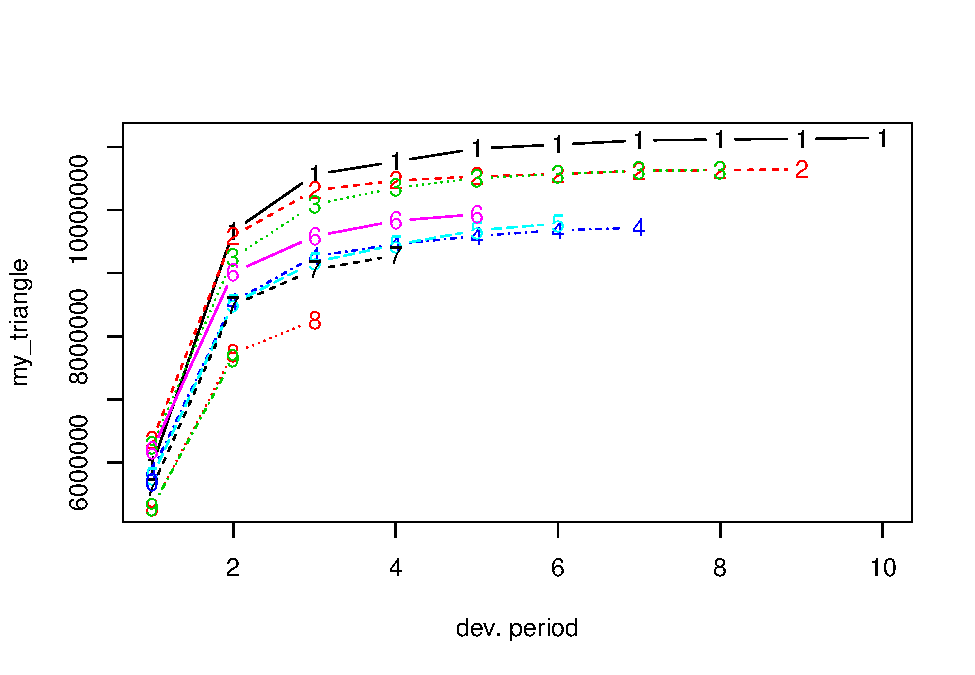
\includegraphics[width=0.8\linewidth]{LossDataAnalytics_files/figure-latex/plottriangle-1} 

}

\caption{Claim Development by Occurrence Year}\label{fig:plottriangle}
\end{figure}

Alternatively, the \texttt{lattice} argument creates one plot per
occurrence year.

\begin{Shaded}
\begin{Highlighting}[]
\KeywordTok{plot}\NormalTok{(my_triangle, }\DataTypeTok{lattice =} \OtherTok{TRUE}\NormalTok{)}
\end{Highlighting}
\end{Shaded}

\begin{center}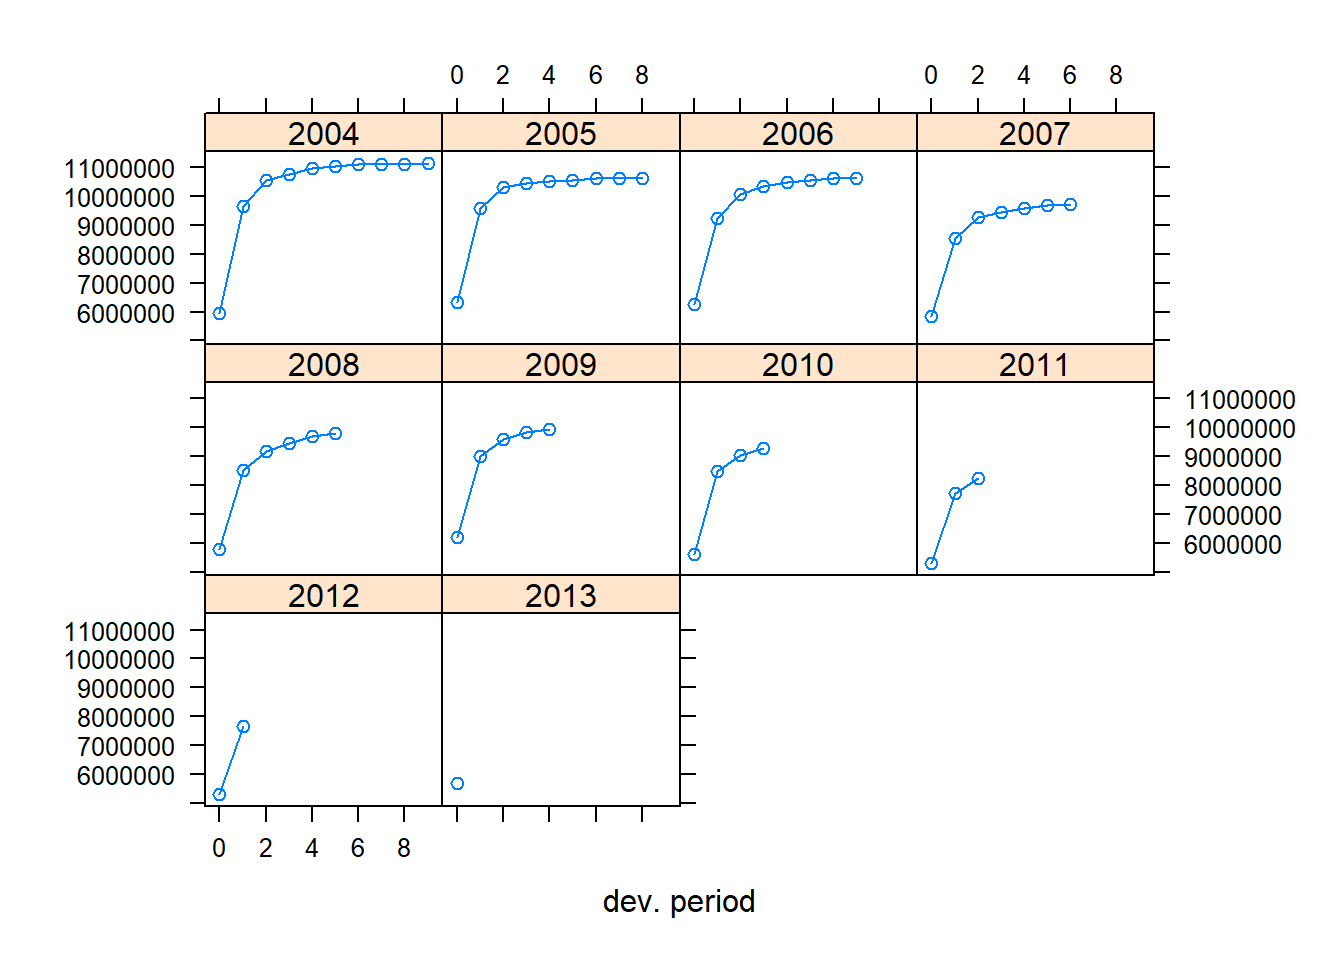
\includegraphics[width=0.8\linewidth]{LossDataAnalytics_files/figure-latex/plot_triangle_lattice-1} \end{center}

Instead of plotting the cumulative triangle stored in
\texttt{my\_triangle}, we can plot the incremental run-off triangle.

\begin{Shaded}
\begin{Highlighting}[]
\KeywordTok{plot}\NormalTok{(my_triangle_incr)}
\end{Highlighting}
\end{Shaded}

\begin{center}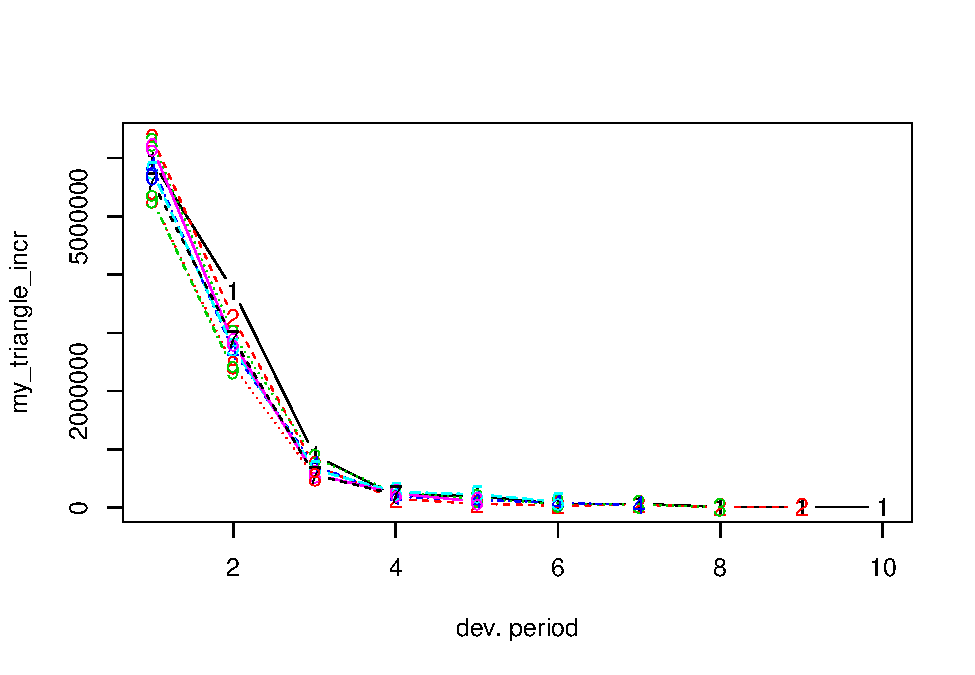
\includegraphics[width=0.8\linewidth]{LossDataAnalytics_files/figure-latex/plot_triangle_incr-1} \end{center}

\begin{Shaded}
\begin{Highlighting}[]
\KeywordTok{plot}\NormalTok{(my_triangle_incr, }\DataTypeTok{lattice =} \OtherTok{TRUE}\NormalTok{)}
\end{Highlighting}
\end{Shaded}

\begin{center}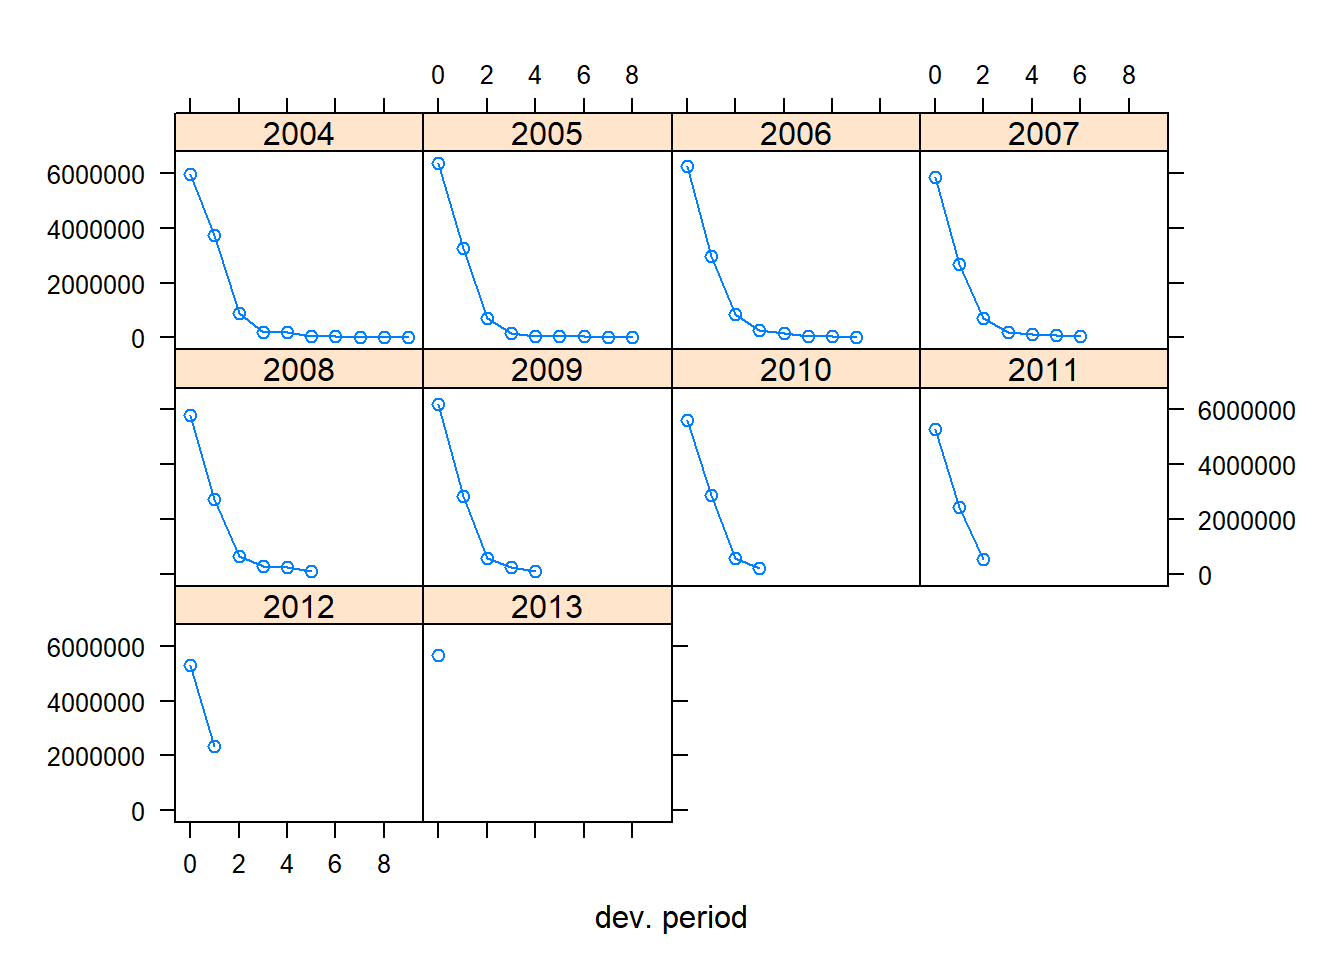
\includegraphics[width=0.8\linewidth]{LossDataAnalytics_files/figure-latex/plot_triangle_incr-2} \end{center}

\section{The Chain-Ladder}\label{S:Chain-ladder}

The most widely used method to estimate outstanding loss reserves is the
so-called chain-ladder method. The origins of this method are obscure
but was firmly entrenched in practical applications by the early 1970's,
\citet{taylor1986claims}. As will be seen, the name refers to the
chaining of a sequence of (year-to-year development) factors into a
ladder of factors; immature losses climb toward maturity when multiplied
by this concatenation of ratios, hence the apt description
\emph{chain-ladder method.} We will start with exploring the
chain-ladder method in its deterministic or algorithmic version, hence
without making any stochastic assumptions. Then we will describe Mack's
distribution-free chain-ladder model.

\subsection{The Deterministic Chain-Ladder}\label{S:DeterministicCL}

The deterministic chain-ladder method focuses on the run-off triangle in
cumulative form. Recall that a cell \((i,j)\) in this triangle displays
the cumulative amount paid up until development period \(j\) for claims
that occurred in year \(i\). The chain-ladder method assumes that
\textbf{development factors} \(f_j\) (also called age-to-age factors,
link ratios or chain-ladder factors) exist such that

\[
C_{i,j+1} = f_j \times C_{i,j}.
\]

Thus, the development factor tells you how the cumulative amount in
development year \(j\) grows to the cumulative amount in year \(j+1\).
We highlight the cumulative amount in period 0 in \textcolor{blue} and
the cumulative amount in period 1 in \textcolor{red} on the Figure
\ref{fig:tikz-cum-triangle-cl1} taken from \citet{WuthrichMerz2008}
(Table 2.2, also used in \citet{WuthrichMerz2015}, Table 1.4).

\begin{figure}

{\centering 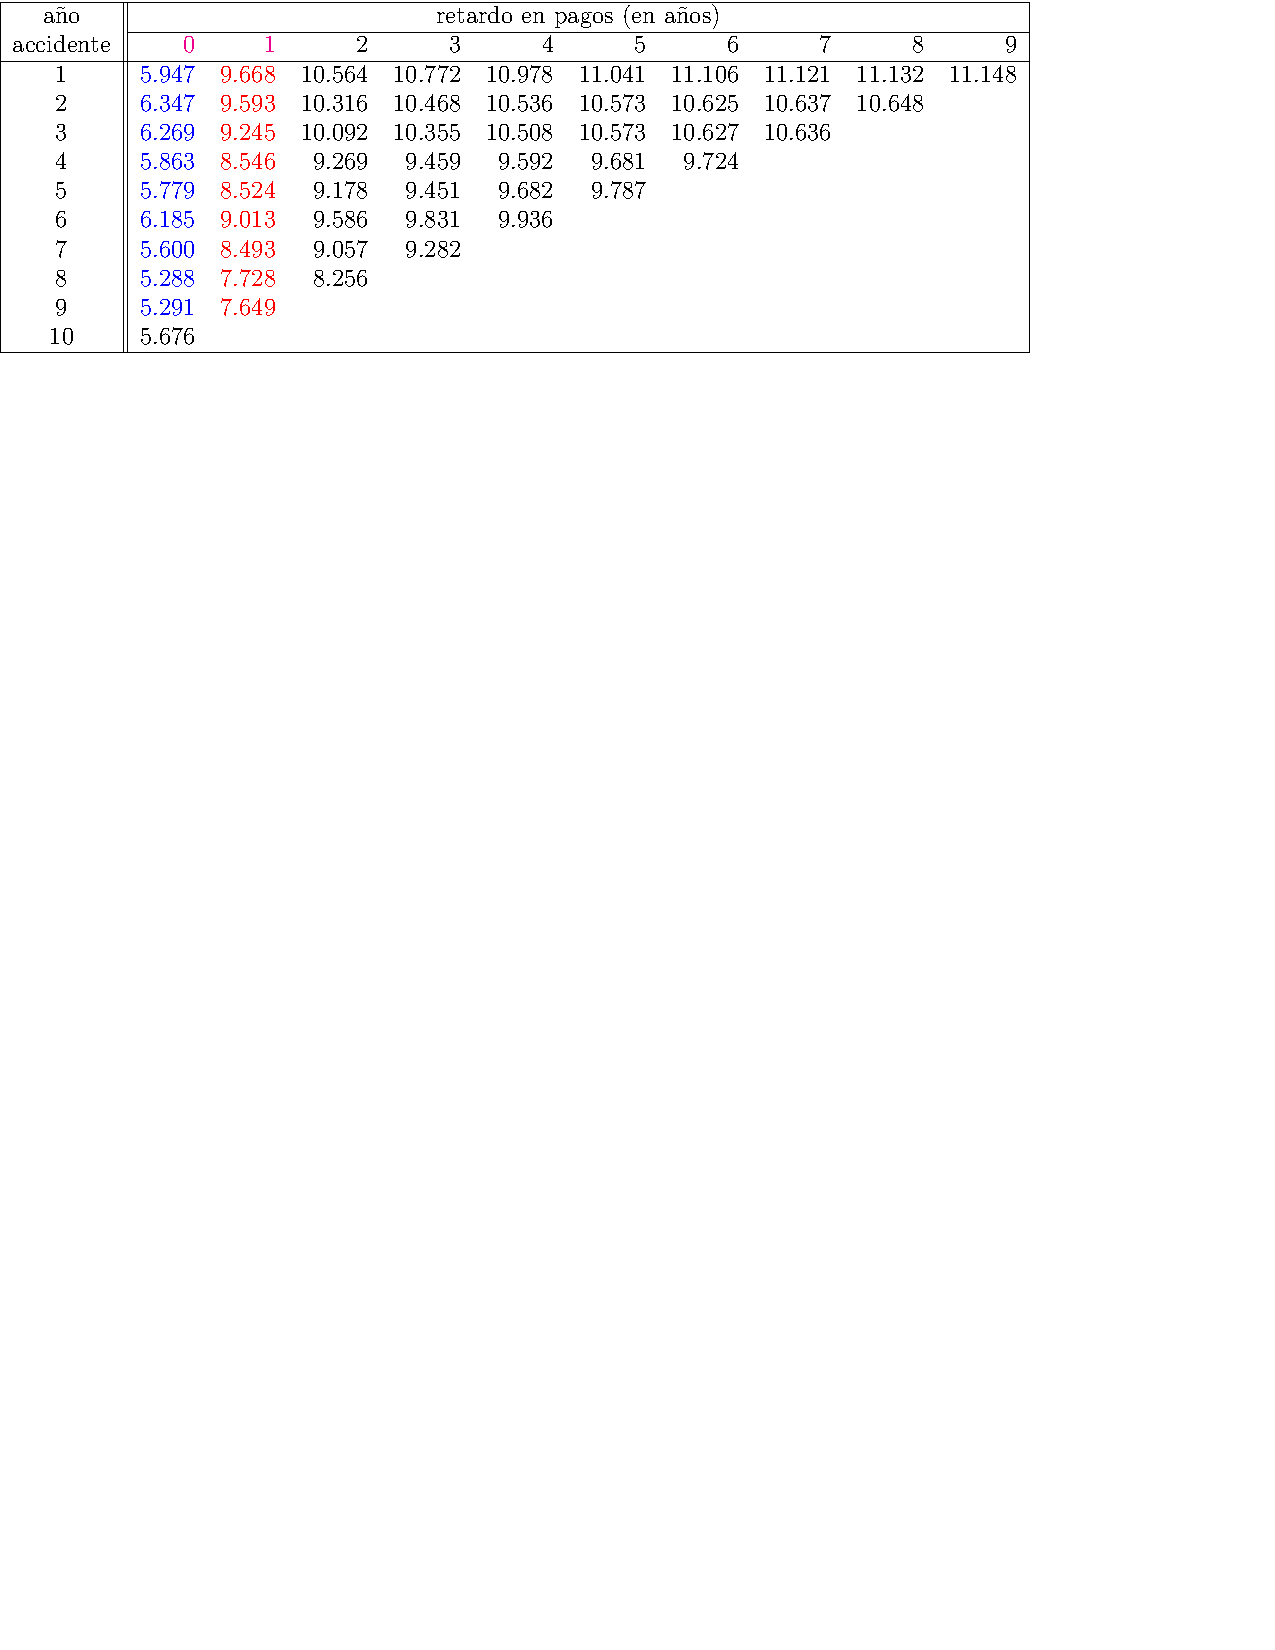
\includegraphics{LossDataAnalytics_files/figure-latex/tikz-cum-triangle-cl1-1} 

}

\caption{A run-off triangle with cumulative payment data highlighting the cumulative amount in period 0 in blue and the cumulative amount in period 1 in red. Source: @WuthrichMerz2008, Table 2.2.}\label{fig:tikz-cum-triangle-cl1}
\end{figure}

The chain-ladder method then presents an intuitive recipe to estimate or
calculate these development factors. Since the first development factor
\(f_0\) describes the development of the cumulative claim amount from
development period 0 to development period 1, it can be estimated as the
ratio of the cumulative amounts in red and the cumulative amounts in
blue, highlighted in the Figure \ref{fig:tikz-cum-triangle-cl1}. In math
notation we then obtain the following estimate \(\hat{f}_0^{CL}\) for
the first development factor \(f_0\), given observations
\(\mathcal{D}_I\):

\[
\hat{f}^{CL}_{\color{magenta}{0}} = \frac{\sum_{i=1}^{10-\color{magenta}{0}-1} \color{red}{C_{i,\color{magenta}{0}+1}}}{\sum_{i=1}^{10-\color{magenta}{0}-1} \color{blue}{C_{i\color{magenta}{0}}}}= 1.4925.
\]

Note that the index \(i\), used in the sums in the numerator and
denominator, runs from the first occurrence period (1) to the last
occurrence period (9) for which both development periods 0 and 1 are
observed. As such, this development factor measures how the data in blue
grow to the data in red, averaged across all occurrence periods for
which both periods are observed. The chain-ladder method then uses this
development factor estimator to predict the cumulative amount
\(C_{10,1}\) (i.e.~the cumulative amount paid up until and including
development year 1 for accidents that occurred in year 10). This
prediction is obtained by multiplying the most recent observed
cumulative claim amount for occurrence period 10 (i.e. \(C_{10,0}\) with
development period 0) with the estimated development factor
\(\hat{f}^{CL}_0\):

\[
\hat{C}_{10, 1} = C_{10,0} \cdot \hat{f}^{CL}_0 = 5,676\cdot 1.4925=8,471.
\] Going forward with this reasoning, the next development factor
\(f_1\) can be estimated. Since \(f_1\) captures the development from
period 1 to period 2, it can be estimated as the ratio of the numbers in
red and the numbers in blue as highlighted in Figure
\ref{fig:tikz-cum-triangle-cl2}.

\begin{figure}

{\centering 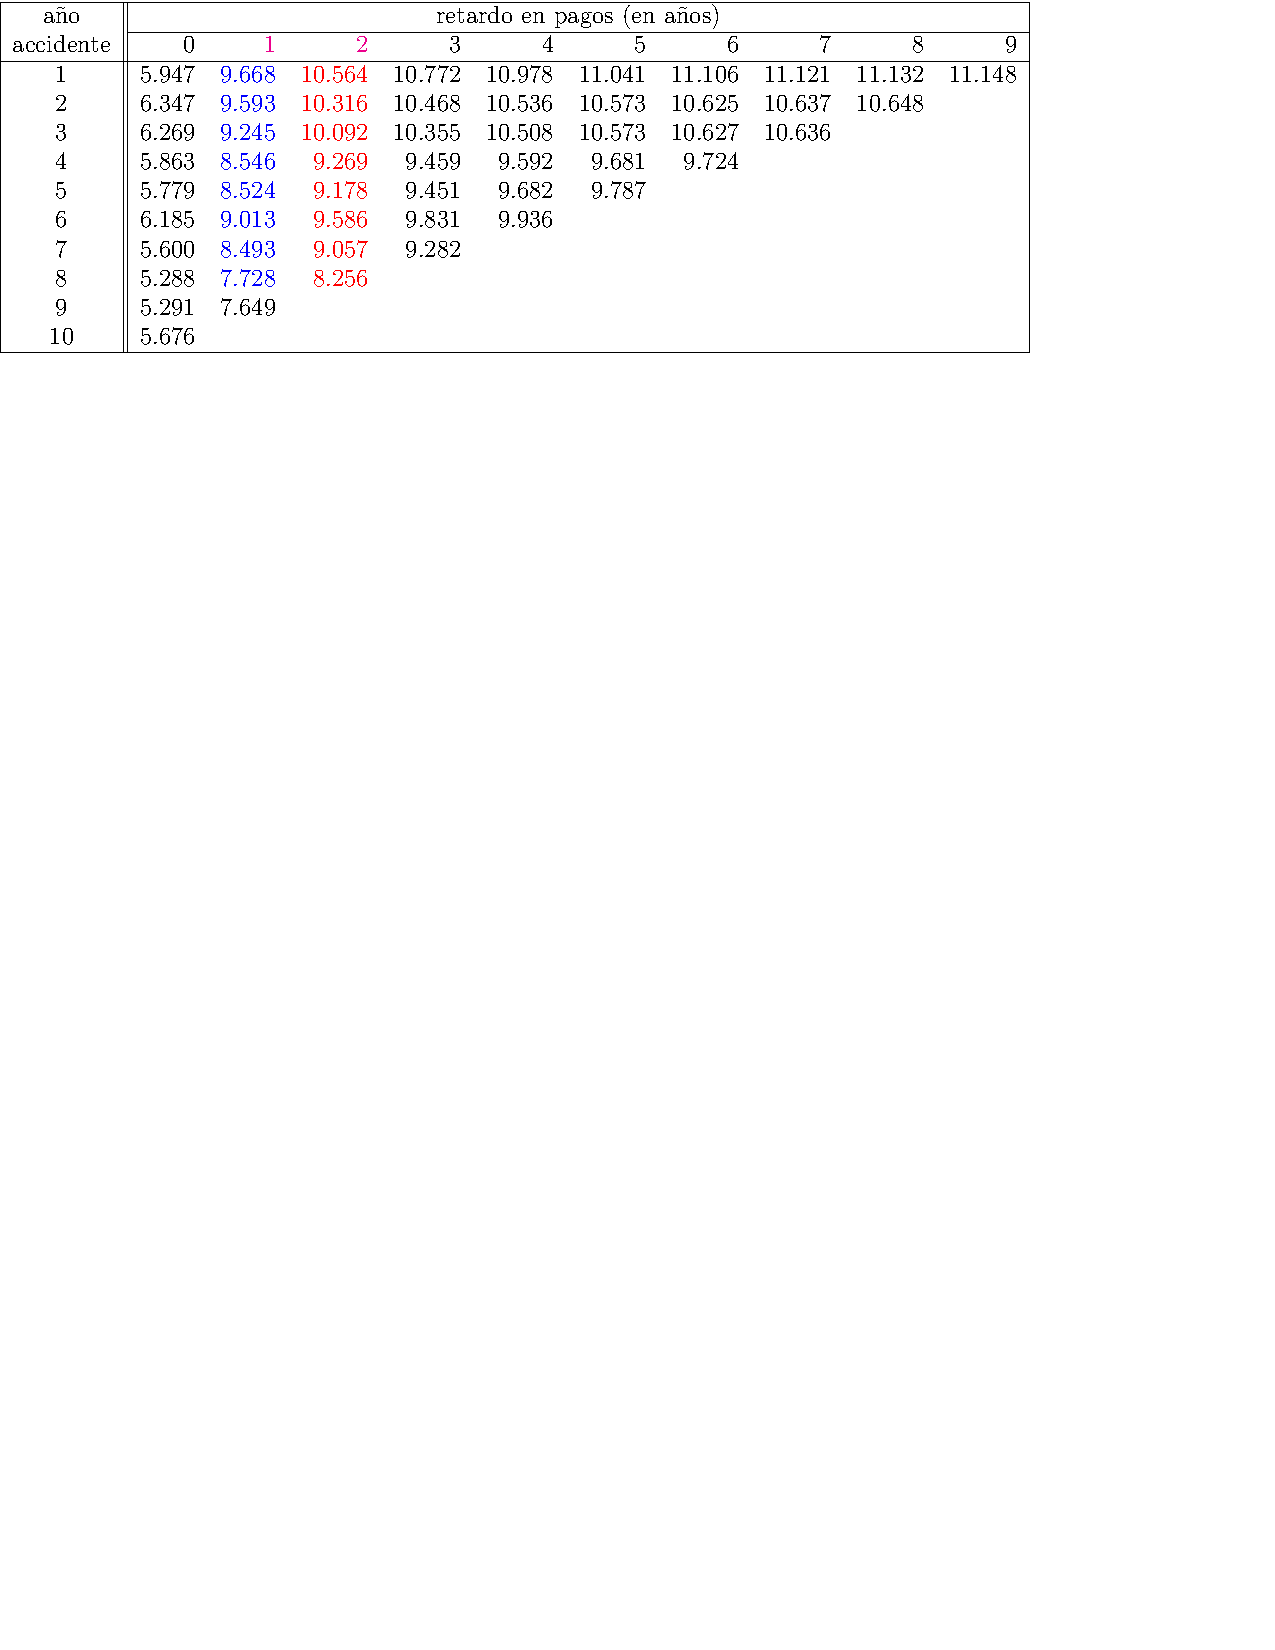
\includegraphics{LossDataAnalytics_files/figure-latex/tikz-cum-triangle-cl2-1} 

}

\caption{A run-off triangle with cumulative payment data highlighting the cumulative amount in period 1 in blue and the cumulative amount in period 2 in red. Source: @WuthrichMerz2008, Table 2.2.}\label{fig:tikz-cum-triangle-cl2}
\end{figure}

The mathematical notation of the estimate \(\hat{f}_1^{CL}\) for the
next development factor \(f_1\), given observations \(\mathcal{D}_I\),
equals:

\[
\hat{f}^{CL}_{\color{magenta}{1}} = \frac{\sum_{i=1}^{10-\color{magenta}{1}-1} \color{red}{C_{i,\color{magenta}{1}+1}}}{\sum_{i=1}^{10-\color{magenta}{1}-1} \color{blue}{C_{i\color{magenta}{1}}}}=1.0778.
\] Consequently, this factor measures how the cumulative paid amount in
development period 1 grows to period 2, averaged across all occurrence
periods for which both periods are observed. The index \(i\) now runs
from period 1 to 8, since these are the occurrence periods for which
both development periods 1 and 2 are observed. This estimate for the
second development factor is then used to predict the missing,
unobserved cells in development period 2:

\[
\begin{array}{rl}
\hat{C}_{10,2} &= C_{10,0} \cdot \hat{f}^{CL}_0 \cdot \hat{f}_1^{CL} = \hat{C}_{10,1} \cdot \hat{f}_1^{CL} = 8,471 \cdot 1.0778 = 9,130 \\
\hat{C}_{9,2}  &= C_{9,1} \cdot \hat{f}^{CL}_1 = 7,649 \cdot 1.0778 = 8,244.
\end{array}
\] Note that for \(\hat{C}_{10,2}\) you actually use the estimate
\(\hat{C}_{10,1}\) and multiply it with the estimated development factor
\(\hat{f}_1^{CL}\).

We continue analogously and obtain following predictions, printed in
italics in the Figure \ref{fig:tikz-cum-triangle-cl3}:

\begin{figure}

{\centering 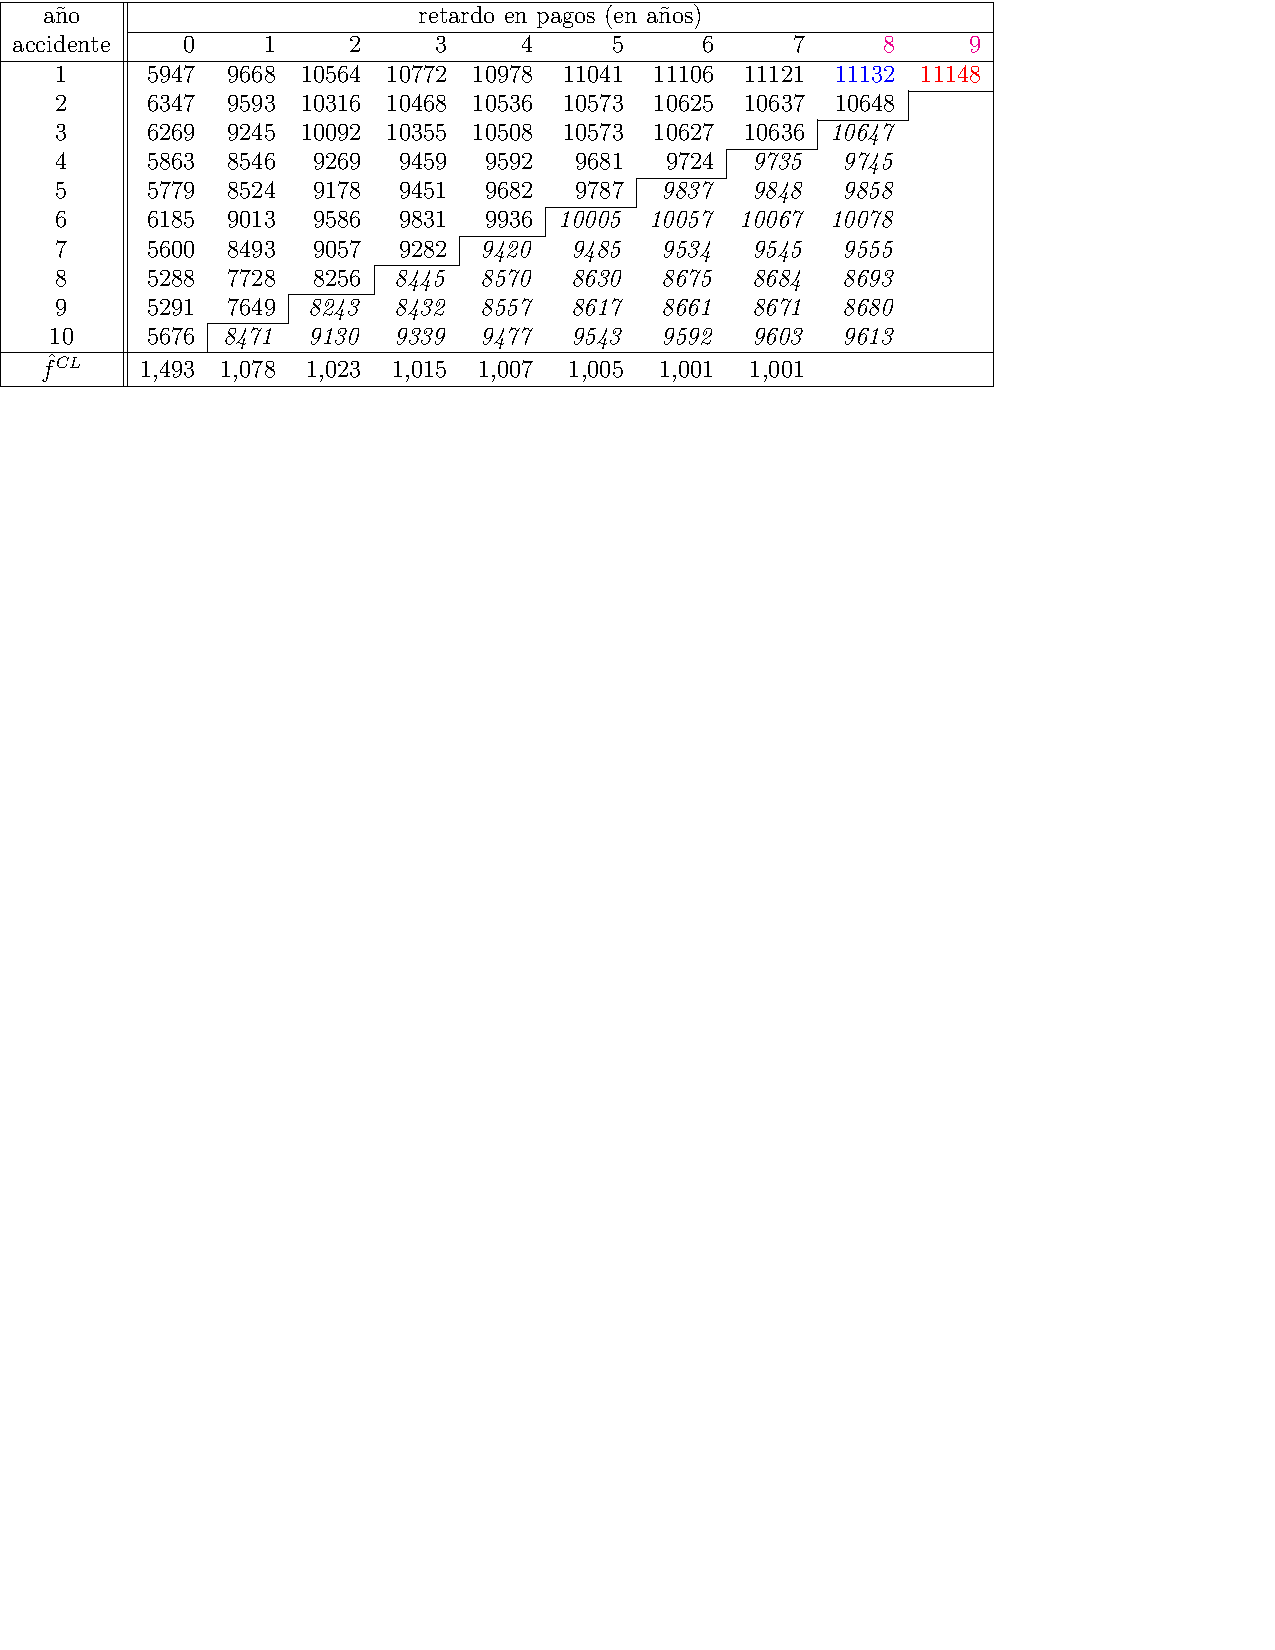
\includegraphics{LossDataAnalytics_files/figure-latex/tikz-cum-triangle-cl3-1} 

}

\caption{A run-off triangle with cumulative payment data including predictions in italic. Source: [@WuthrichMerz2008], Table 2.2.}\label{fig:tikz-cum-triangle-cl3}
\end{figure}

Eventually we need to estimate the values in the final column. The last
development factor \(f_8\) measures the growth from development period 8
to development period 9 in the triangle. Since only the first row in the
triangle has both cells observed, this last factor is estimated as the
ratio of the value in red and the value in blue in Figure
\ref{fig:tikz-cum-triangle-cl3b}.

\begin{figure}

{\centering 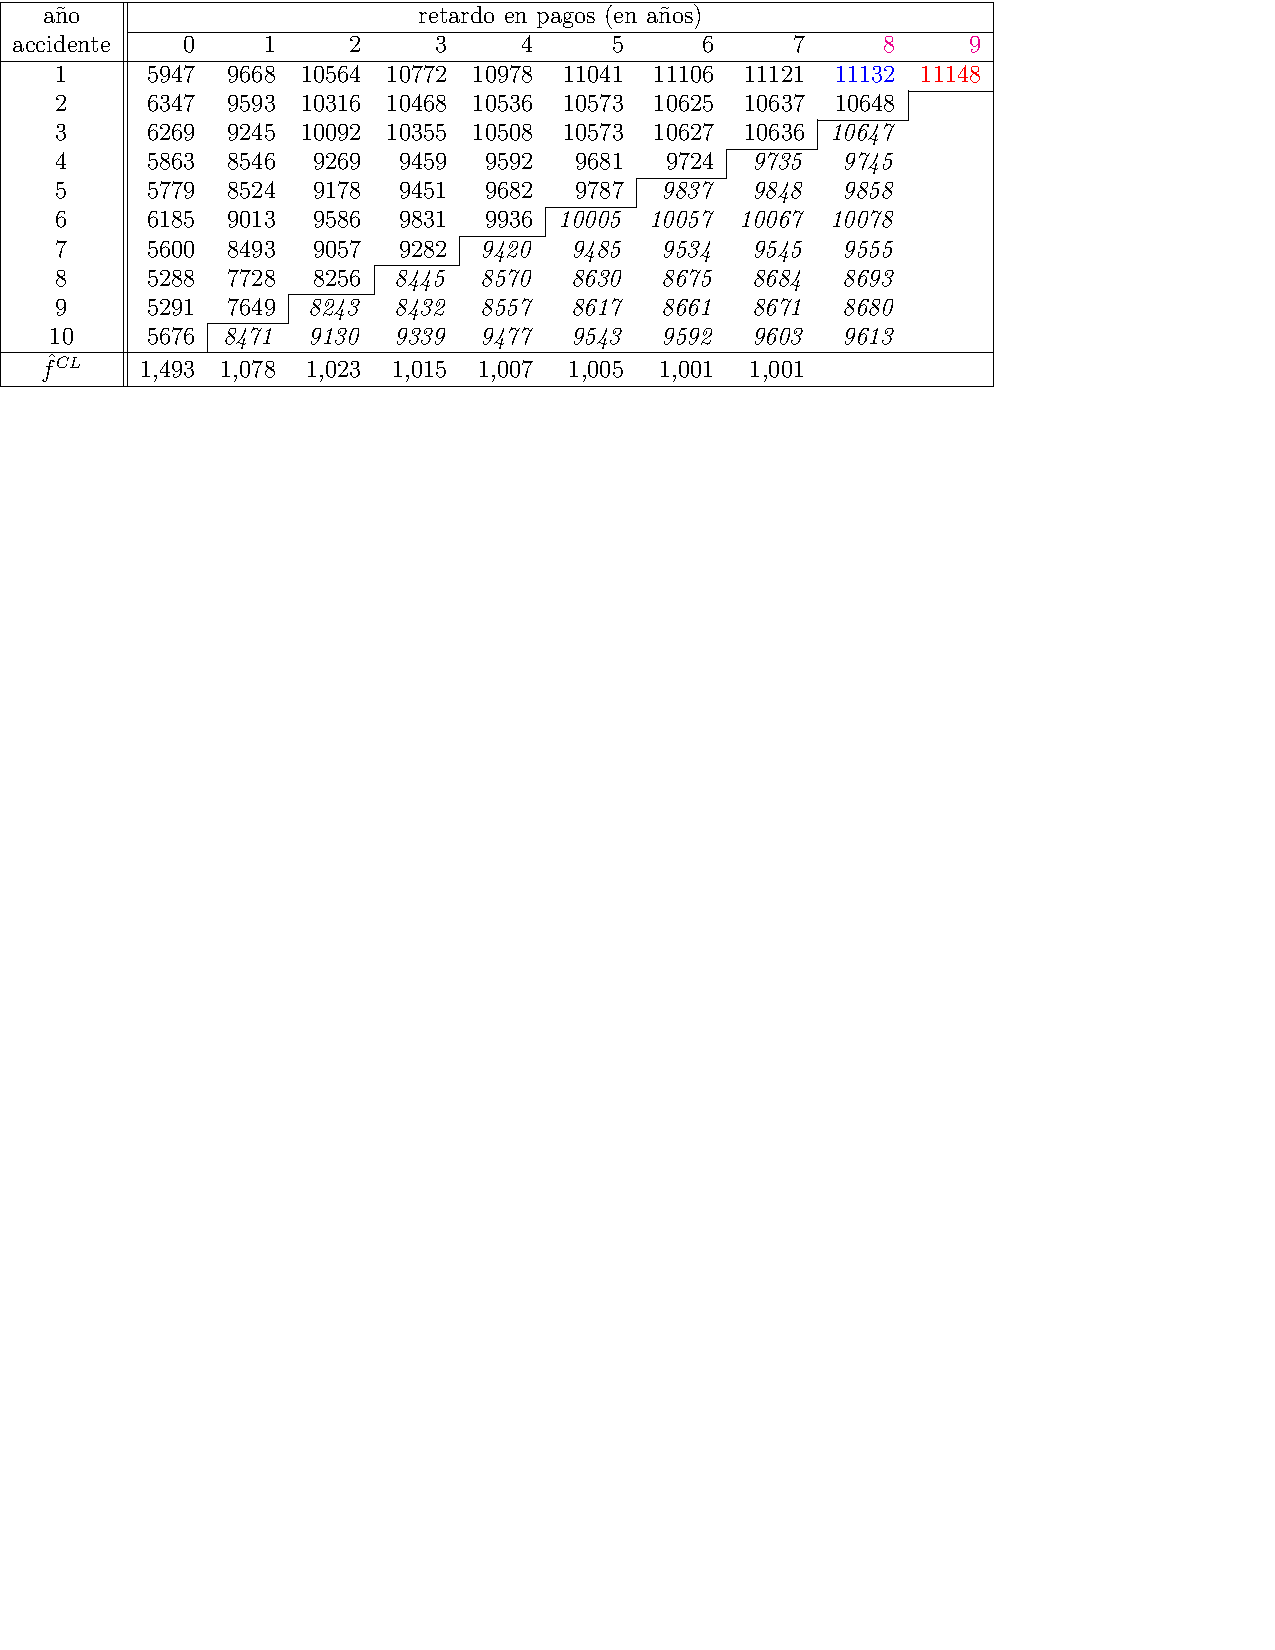
\includegraphics{LossDataAnalytics_files/figure-latex/tikz-cum-triangle-cl3b-1} 

}

\caption{A run-off triangle with cumulative payment data highlighting the cumulative amount in period 8 in blue and the cumulative amount in period 9 in red. Source: [@WuthrichMerz2008], Table 2.2.}\label{fig:tikz-cum-triangle-cl3b}
\end{figure}

Given observations \(\mathcal{D}_I\), this factor estimate
\(\hat{f}^{CL}_{8}\) is equal to:

\[
\hat{f}^{CL}_{\color{magenta}{8}} = \frac{\sum_{i=1}^{10-\color{magenta}{8}-1} \color{red}{C_{i,\color{magenta}{8}+1}}}{\sum_{i=1}^{10-\color{magenta}{8}-1} \color{blue}{C_{i\color{magenta}{8}}}}=1.001.
\] Typically this last development factor is close to 1 and hence the
cash flows paid in the final development period are minor. Using this
development factor estimate, we can now estimate the remaining
cumulative claim amounts in the column by multiplying the values for
development year 8 with this factor.

The general math notation for the chain ladder predictions for the lower
triangle (\(i+j>I\)) is as follows:

\[
\begin{array}{rl}
\hat{C}_{ij}^{CL} &= C_{i,I-i} \cdot \prod_{l=I-i}^{j-1} \hat{f}_l^{CL} \\
\hat{f}_j^{CL} &= \frac{\sum_{i=1}^{I-j-1} C_{i,j+1}}{\sum_{i=1}^{I-j-1} C_{ij}},
\end{array}
\] where \(C_{i,I-i}\) is on the last observed diagonal. It is clear
that an important assumption of the chain-ladder method is that the
proportional developments of claims from one development period to the
next are similar for all occurrence years.

This yields the following Figure \ref{fig:tikz-cum-triangle-cl4}:

\begin{figure}

{\centering 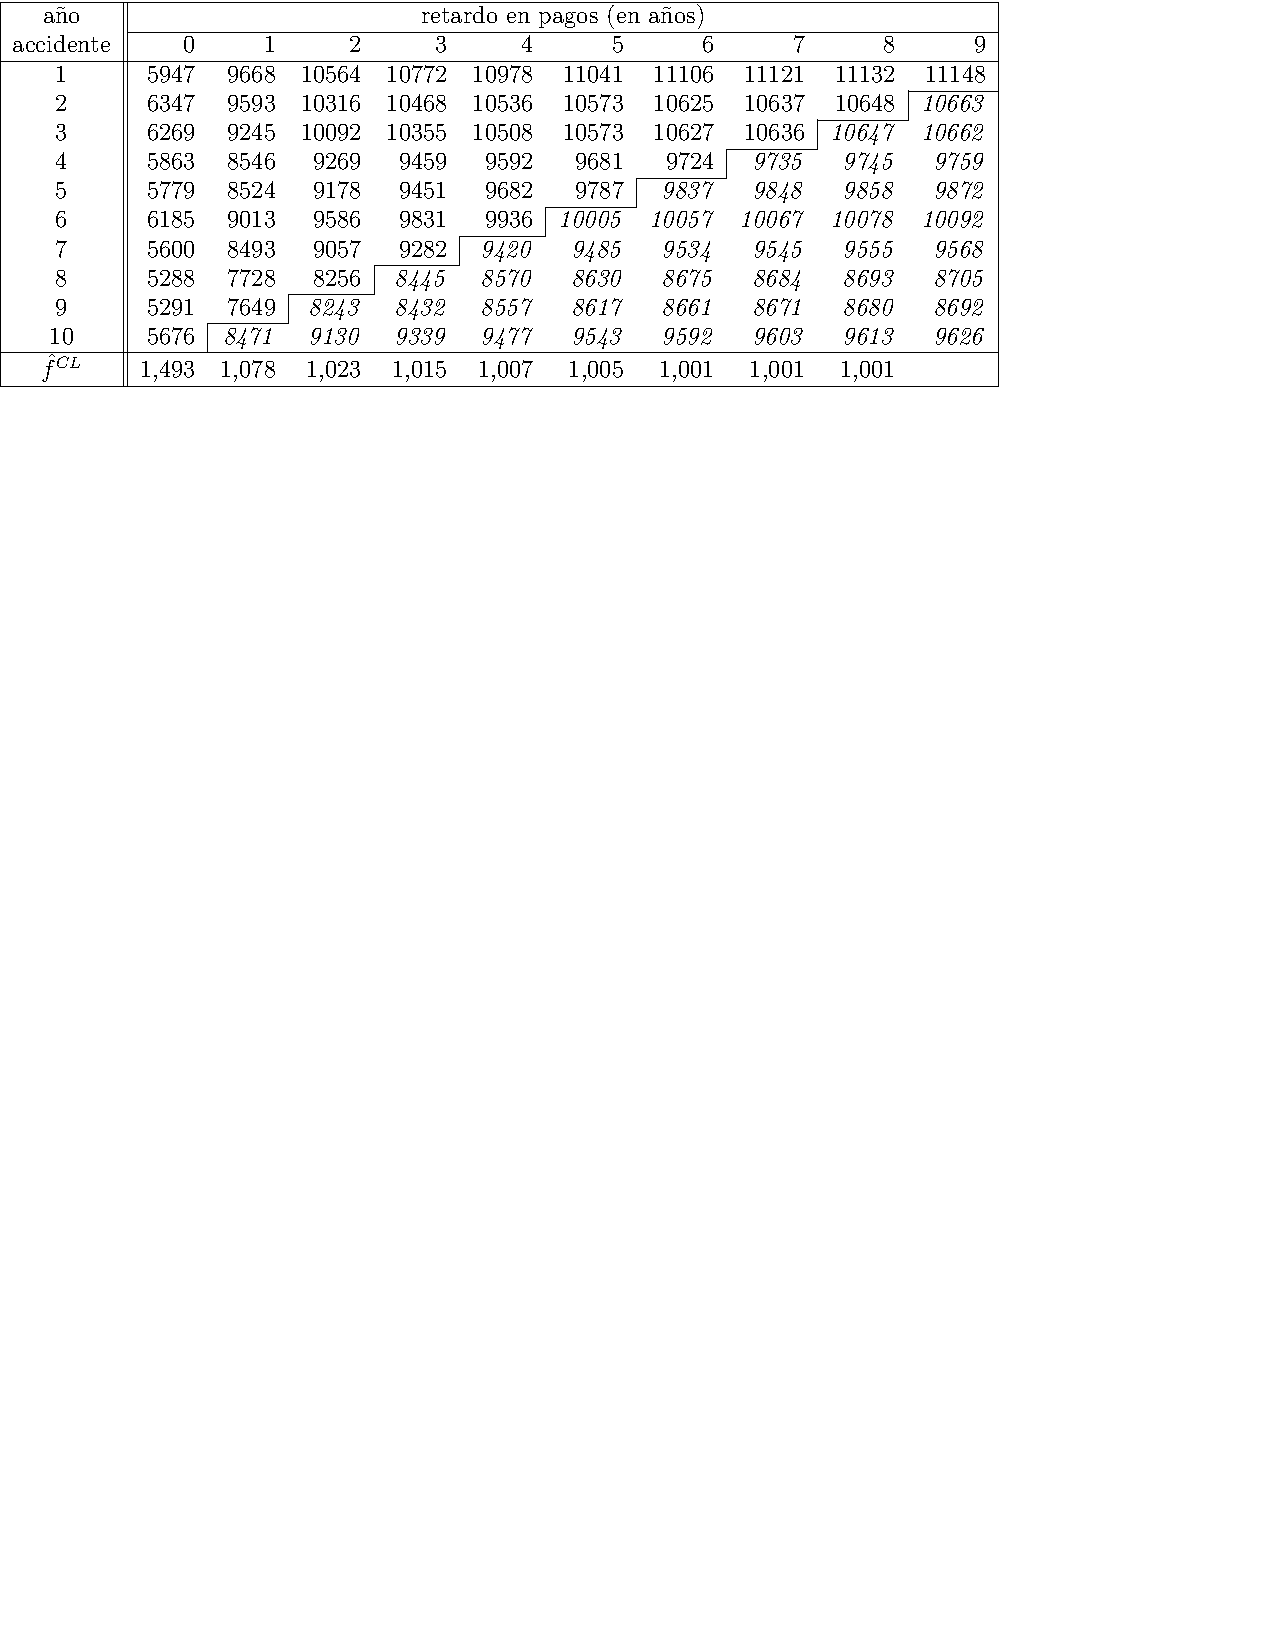
\includegraphics{LossDataAnalytics_files/figure-latex/tikz-cum-triangle-cl4-1} 

}

\caption{A run-off triangle with cumulative payment data including predictions in italic. Source: @WuthrichMerz2008, Table 2.2.}\label{fig:tikz-cum-triangle-cl4}
\end{figure}

The numbers in the last column show the estimates for the ultimate claim
amounts. The estimate for the outstanding claim amount
\(\hat{\mathcal{R}}_i^{CL}\) for a particular occurrence period
\(i=I-J+1,\ldots, I\) is then given by the difference between the
ultimate claim amount and the cumulative amount as observed on the most
recent diagonal:

\[
\hat{\mathcal{R}}_i^{CL} =\hat{C}_{iJ}^{CL}-C_{i,I-i}.
\] This is the chain-ladder estimate for the reserve necessary to
fulfill future liabilities with respect to claims that occurred in this
particular occurrence period. These reserves per occurrence period and
for the total summed over all occurrence periods are summarized in
Figure \ref{fig:tikz-cum-triangle-cl5}.

\begin{figure}

{\centering 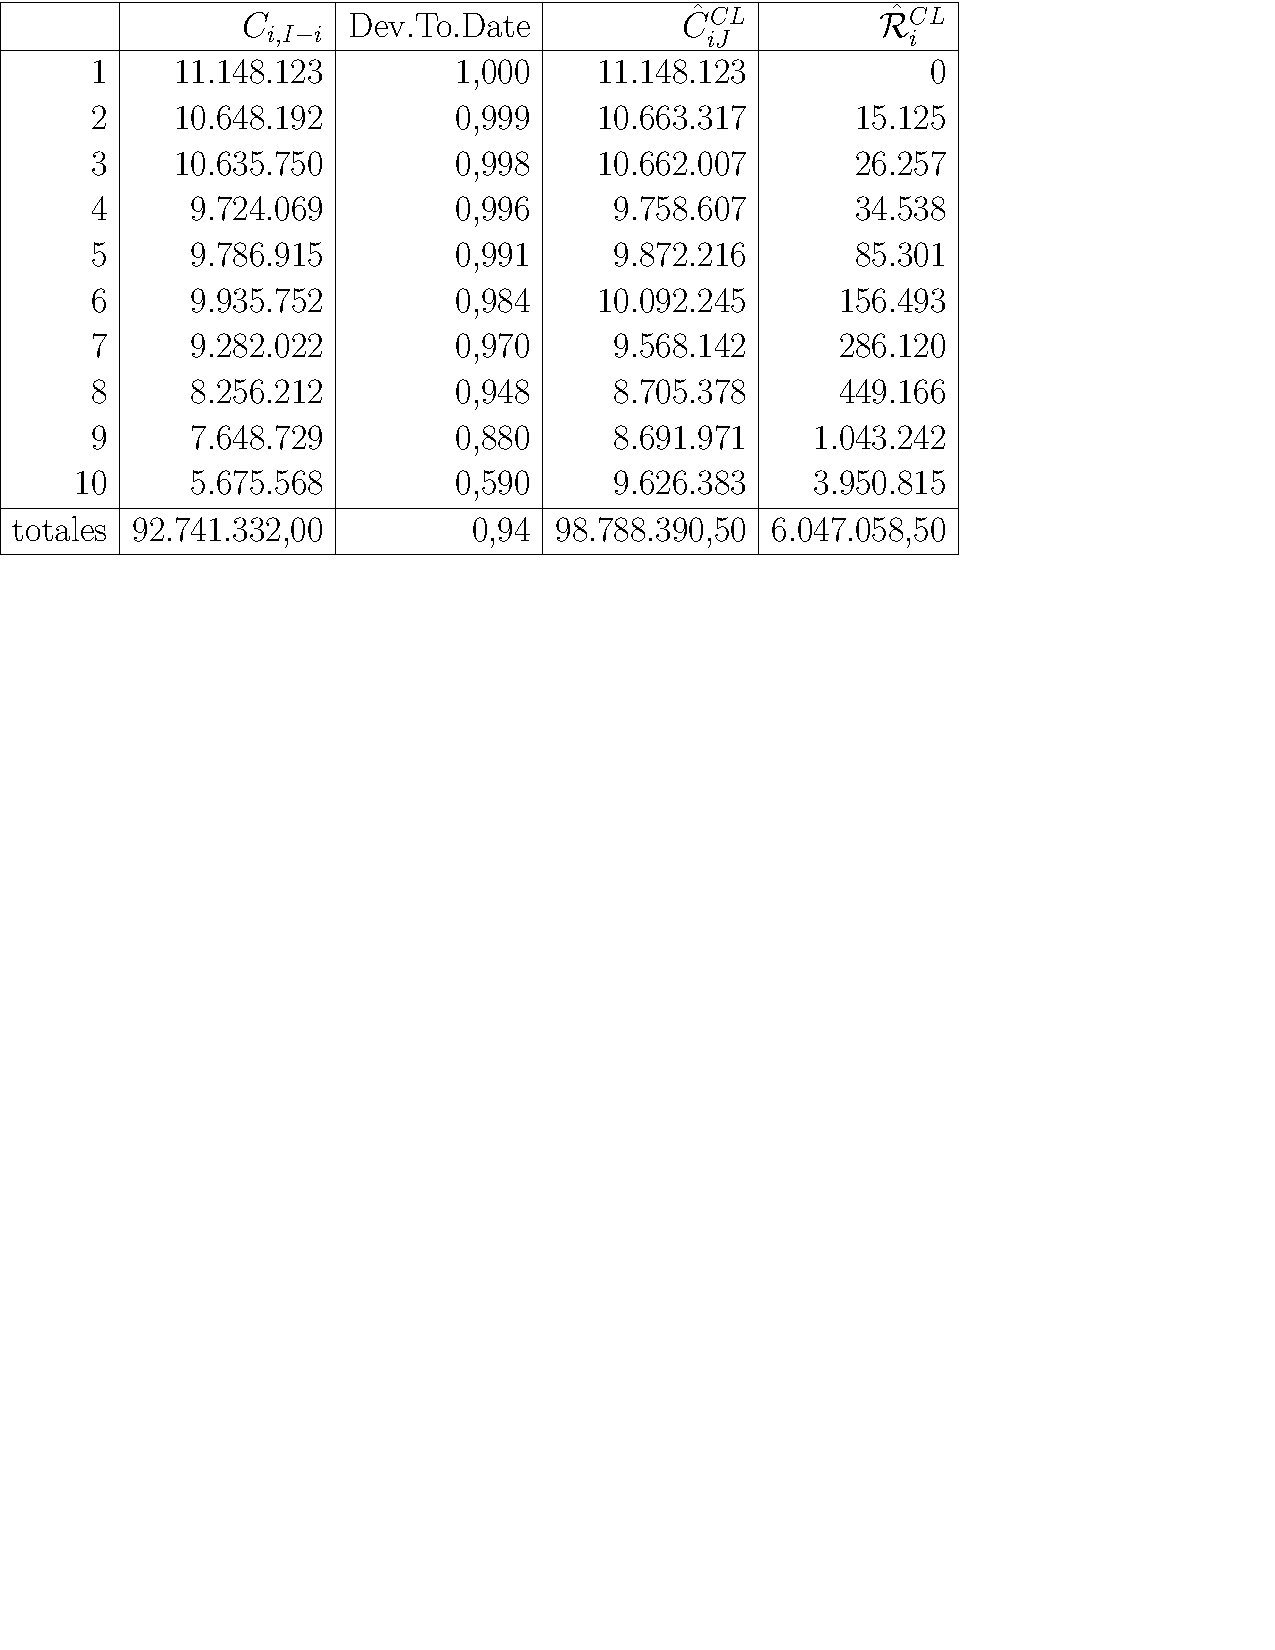
\includegraphics{LossDataAnalytics_files/figure-latex/tikz-cum-triangle-cl5-1} 

}

\caption{Reserves per occurence period and for total}\label{fig:tikz-cum-triangle-cl5}
\end{figure}

\subsection{Mack's Distribution-Free Chain-Ladder
Model}\label{macks-distribution-free-chain-ladder-model}

At this stage, the traditional chain-ladder method provides a point
estimator \(\hat{C}^{CL}_{iJ}\) for the forecast of \(C_{iJ}\), using
the information \(\mathcal{D}_I\). Since the chain-ladder method is a
purely deterministic and intuitively natural algorithm to complete a
run-off triangle, we are not able to determine how reliable that point
estimator is or to model the variation of the future payments. To answer
such questions an underlying stochastic model that reproduces the
chain-ladder reserve estimates is needed.

In this section we will focus on the distribution-free chain-ladder
model as an underlying stochastic model, introduced in \citet{Mack1993}.
This method allows us to estimate the standard errors of the
chain-ladder predictions. In the next Section \ref{S:GLMs}, generalized
linear models are used to develop a fully stochastic approach for
predicting the outstanding reserve.

In Mack's approach the following conditions (without assuming a
distribution) hold:

\begin{itemize}
\item
  Cumulative claims \((C_{ij})_{j=0,\ldots,J}\) are independent over
  different occurrence periods \(i\).
\item
  There exist fixed constants \(f_0, \ldots, f_{J-1}\) and
  \(\sigma^2_0,\ldots, \sigma^2_{J-1}\) such that for all
  \(i=1,\ldots, I\) and \(j=0,\ldots,J-1\):
\end{itemize}

\[
\begin{array}{rl}
E[C_{i,j+1}|C_{i0},\ldots,C_{ij}] &= f_j \cdot C_{ij} \\
\text{Var}(C_{i,j+1}|C_{ij}) &= \sigma^2_j \cdot C_{ij}.
\end{array}
\]

This means that the cumulative claims \((C_{ij})_{j=0,\ldots,J}\) are
Markov processes (in the development periods \(j\)) and hence the future
only depends on the present.

Under these assumptions, the expected value of the ultimate claim amount
\(C_{i,J}\), given the available data in the upper triangle, is the
cumulative amount on the most recent diagonal (\(C_{i, I-1}\))
multiplied with appropriate development factors \(f_j\). In mathematical
notation we obtain for known development factors \(f_j\) and
observations \(\mathcal{D}_I\):

\[
E[C_{iJ}|\mathcal{D}_I] = C_{i,I-i} \prod_{j=I-i}^{J-1} f_j.
\] This is exactly what the deterministic chain-ladder method does, as
explained in Section \ref{S:DeterministicCL}. In practice, the
development factors are not known and need to be estimated from the data
that is available in the upper triangle. In Mack's approach we obtain
exactly the same expression for estimating the development factors
\(f_j\) at time \(I\) as in the deterministic chain-ladder algorithm:

\[
\hat{f}_j^{CL} =\frac{\sum_{j=1}^{I-j-1} C_{i,j+1}}{\sum_{i=1}^{I-j-1} C_{ij}}.
\] The predictions for the cells in the lower triangle (i.e.~for cells
\$C\_\{i,j\} \$where \(i+j>I\)) are then obtained by replacing the
unknown factors \(f_j\) by their corresponding estimates
\(\hat{f}_j^{CL}\):

\[
\hat{C}^{CL}_{ij} = C_{i,I-i}\prod_{l=I-i}^{j-1} \hat{f}_l^{CL}.
\]

To quantify the prediction error that comes with the chain-ladder
predictions, Mack also introduced variance parameters \(\sigma^2_j\). To
gain insight in the estimation of these variance parameters, so-called
individual development factors \(f_{i,j}\) are introduced (which are
specific to occurrence period \(i\)):

\[
f_{i,j} = \frac{C_{i,j+1}}{C_{ij}}.
\] These individual development also describe how the cumulative amount
grows from period \(j\) to period \(j+1\), but they consider the ratio
of only two cells (instead of taking the ratio of two sums over all
available occurrence periods). Note that the development factors can be
written as a weighted average of individual development factors:

\[
\hat{f}_j^{CL} = \sum_{i=1}^{I-j-1} \frac{C_{ij}}{\sum_{i=1}^{I-j-1} C_{ij}} f_{i,j},
\] where the weights are equal to the cumulative claims \(C_{ij}\).

Let us now estimate the variance parameters \(\sigma^2\) by writing
Mack's variance assumption in equivalent ways. First, the variance of
the ratio of \(C_{i,j+1}\) and \(c_{i,j}\) conditional on
\(C_{i,0},\ldots, C_{i,j}\) is proportional to the inverse of
\(C_{i,j}\):

\[
\text{Var}[C_{i,j+1}/C_{ij}|C_{i0},\ldots,C_{ij}] ~ \propto ~ \frac{1}{C_{ij}}.
\]

This reminds us of a typical \emph{weighted least squares} setting where
the weights are the inverse of the variability of a response. Therefore,
a more volatile or imprecise response variable will get less weight. The
\(C_{i,j}\) play the role of the weights. Using the unknown variance
parameter \(\sigma^2_j\) this variance assumption can be written as:

\[
\text{Var}[C_{i,j+1}|C_{i0},\ldots,C_{ij}] = \sigma^2_j \cdot C_{ij},
\] The connection with weighted least squares then directly leads to an
unbiased estimate for the unknown variance parameter \(\sigma^2_j\) in
the form of a weighted residual sum of squares:

\[
\hat{\sigma}^2_j = \frac{1}{I-j-2}\sum_{i=1}^{I-j-1} C_{ij}\left(\frac{C_{i,j+1}}{C_{ij}}-\hat{f}_j^{CL}\right)^2.
\] The weights are again equal to \(C_{i,j}\) and the residuals are the
differences between the ratios \(C_{i,j+1}/C_{i,j}\) and the individual
development factors.

We now have all ingredients required to calibrate the distribution-free
chain-ladder model to the data. The next step is then to analyze the
prediction uncertainty and the prediction error. Hereto we use the
chain-ladder predictor where we replace the unknown development factors
with their estimators:

\[
\hat{C}_{iJ}^{CL} = C_{i,I-i} \prod_{l=I-i}^{J-1} \hat{f}_l^{CL}
\]

We use this expression either as an estimator for the conditional
expectation of the ultimate claim amount (given the observed upper
triangle) or as a predictor for the ultimate claim amount as a random
variable (given the observed upper triangle).

In statistics the simplest measure to analyze the uncertainty that comes
with a point estimate or prediction is the \emph{Mean Squared Error of
Prediction} (\emph{MSEP}). Here we consider a conditional \emph{MSEP},
conditional on the data observed in the upper triangle:

\[
MSEP_{C_{iJ}|\mathcal{D}_I}\left(\hat{C}_{iJ}^{CL}\right) = E\left[\left(C_{iJ}-\hat{C}_{iJ}^{CL}\right)^2|\mathcal{D}_I\right]. 
\] This conditional \emph{MSEP} measures:

\begin{itemize}
\tightlist
\item
  the distance between the (true) ultimate claim \(C_{iJ}\) and its
  chain-ladder predictor \(\hat{C}_{iJ}^{CL}\) at time \(I\), and
\item
  the total prediction uncertainty over the entire run-off of the
  nominal ultimate claim \(C_{iJ}\). It does not consider time value of
  money, a risk margin nor any dynamics in its developments.
\end{itemize}

The \emph{MSEP} that comes with the estimate for the ultimate cumulative
claim amount is equal to the \emph{MSEP} that measures the squared
distance between the true and the estimated reserve:

\[
\begin{array}{rl}
MSEP_{\hat{\mathcal{R}}^{I}_{i}|\mathcal{D}_I}(\hat{\mathcal{R}}^{I}_i) &= E[(\hat{\mathcal{R}}^I_i-\mathcal{R}^I_i)^2|\mathcal{D}_I] \\
&= E[(\hat{C}^{CL}_{iJ}-C_{iJ})^2|\mathcal{D}_I] = MSEP(\hat{C}_{iJ}). 
\end{array}
\] The reason for this equivalence is the fact that the reserve is the
ultimate claim amount minus the most recently observed claim amount. The
latter is observed and used in both \(\mathcal{R}^I_i\) and
\(\hat{\mathcal{R}}^I_i\).

It is interesting to decompose this \emph{MSEP} into a component that
captures \emph{process variance} and a component that captures
\emph{parameter estimation variance}:

\[
\begin{array}{rl}
MSEP_{C_{iJ|\mathcal{D}_I}}\left(\hat{C}_{iJ}^{CL}\right) &=
E\left[ \left( C_{iJ} - \hat{C}_{iJ} \right)^2 | \mathcal{D}_I\right] \\
&= \text{Var}(C_{iJ}|\mathcal{D}_I) + \left( E[C_{iJ}|\mathcal{D}_I]-\hat{C}_{iJ}^{CL} \right)^2 \\
&= \color{magenta}{\text{process variance}} + \color{magenta}{\text{parameter estimation variance}},
\end{array}
\]

for a \(\mathcal{D}_I\) measurable estimator/predictor \(\hat{C}_{iJ}\).
The process variance component captures the volatility or uncertainty in
the random variable \(C_{i,J}\) and the parameter estimation variance
measures the error that arises from replacing the unknown development
factors \(f_j\) with their estimated values. This result follows
immediately from following equality about the variance of a shifted
random variable \(X\) where the shift \(a\) is deterministic:

\[
E(X-a)^2 = \text{Var}(X)+\left[EX-a\right]^2.
\]

Applied to the expression of the \emph{MSEP} you treat \(\hat{C}_{i,J}\)
as fixed because you work conditionally on the data in the upper
triangle and \(\hat{C}_{i,J}\) only uses information from this upper
triangle.

\citet{Mack1993} then derived the important formula for the conditional
\emph{MSEP} in the distribution-free chain-ladder model for a single
occurrence period \(i\):

\[
\widehat{MSEP_{C_{iJ}|\mathcal{D}_I}}  =
\left(\hat{C}_{iJ}^{CL}\right)^2 \sum_{j=I-i}^{J-1} \left[ \frac{\hat{\sigma}_j^2}{(\hat{f}_j^{CL})^2} \left(\frac{1}{\hat{C}^{CL}_{ij}}+\frac{1}{\sum_{n=1}^{I-j-1}C_{nj}}\right)\right].
\]

For the derivation of this popular formula, we refer to his paper. Note
that it is an estimate of the \emph{MSEP} since the unknown parameters
\(f_j\) and \(\sigma_j\) need to be estimated and since the estimation
error cannot be calculated explicitly.

Mack also derived a formula for the \emph{MSEP} for the total reserve,
across all occurrence periods:

\[
\begin{array}{ll}
\widehat{MSEP_{\sum_{i=1}^I \hat{C}^{CL}_{iJ}}}\left( \sum_{i=1}^I \hat{C}^{CL}_{iJ}  \right) \\
 \ \ \ \ \ \sum_{i=1}^I \widehat{MSEP_{C_{iJ}|\mathcal{D}_I}}\left( \hat{C}^{CL}_{iJ} \right)
\color{blue}{+2 \sum_{1\leq i< k \leq I} \hat{C}_{iJ}^{CL} \hat{C}_{kJ}^{CL}
\sum_{j=I-i}^{J-1} \frac{ \hat{\sigma}_j^2/\left( \hat{f}_j^{\text{CL}} \right)^2 }{ \sum_{n=1}^{I-j-1} C_{nj} }}.
\end{array}
\] The result is the sum of the \emph{MSEP}s per occurrence period plus
a covariance term. This covariance term is added because the MSEPs for
different occurrence periods \(i\) use the same parameter estimates
\(\hat{f}_j^{CL}\) of \(f_j\) for different accident years \(i\).

\subsection{R code for Chain-Ladder
Predictions}\label{r-code-for-chain-ladder-predictions}

We use the object \texttt{my\_triangle} of type \texttt{triangle} that
was created in Section \ref{S:Rcode}. The distribution-free chain-ladder
model of \citet{Mack1993} is implemented in the \texttt{ChainLadder}
package \citep{R-chainladder} (as a special form of weighted least
squares) and can be applied on the data \texttt{my\_triangle} to predict
outstanding claim amounts and to estimate the standard error around
those forecasts.

\begin{Shaded}
\begin{Highlighting}[]
\NormalTok{CL <-}\StringTok{ }\KeywordTok{MackChainLadder}\NormalTok{(my_triangle)}
\NormalTok{CL}
\end{Highlighting}
\end{Shaded}

\begin{verbatim}
MackChainLadder(Triangle = my_triangle)

         Latest Dev.To.Date   Ultimate      IBNR Mack.S.E CV(IBNR)
2004 11,148,124       1.000 11,148,124         0        0      NaN
2005 10,648,192       0.999 10,663,318    15,126      716   0.0474
2006 10,635,751       0.998 10,662,008    26,257    1,131   0.0431
2007  9,724,068       0.996  9,758,606    34,538    3,121   0.0904
2008  9,786,916       0.991  9,872,218    85,302    7,654   0.0897
2009  9,935,753       0.984 10,092,247   156,494   33,347   0.2131
2010  9,282,022       0.970  9,568,143   286,121   73,469   0.2568
2011  8,256,211       0.948  8,705,378   449,167   85,400   0.1901
2012  7,648,729       0.880  8,691,971 1,043,242  134,338   0.1288
2013  5,675,568       0.590  9,626,383 3,950,815  410,818   0.1040

                 Totals
Latest:   92,741,334.00
Dev:               0.94
Ultimate: 98,788,397.77
IBNR:      6,047,063.77
Mack.S.E     462,977.83
CV(IBNR):          0.08
\end{verbatim}

\begin{Shaded}
\begin{Highlighting}[]
\KeywordTok{round}\NormalTok{(}\KeywordTok{summary}\NormalTok{(CL)}\OperatorTok{$}\NormalTok{Totals)}
\end{Highlighting}
\end{Shaded}

\begin{verbatim}
             Totals
Latest:    92741334
Dev:              1
Ultimate:  98788398
IBNR:       6047064
Mack S.E.:   462978
CV(IBNR):         0
\end{verbatim}

The development factors are obtained as follows:

\begin{Shaded}
\begin{Highlighting}[]
\KeywordTok{round}\NormalTok{(CL}\OperatorTok{$}\NormalTok{f,}\DataTypeTok{digits =} \DecValTok{4}\NormalTok{)}
\end{Highlighting}
\end{Shaded}

\begin{verbatim}
 [1] 1.4925 1.0778 1.0229 1.0148 1.0070 1.0051 1.0011 1.0010 1.0014 1.0000
\end{verbatim}

We can also print the complete run-off triangle (including predictions).

\begin{Shaded}
\begin{Highlighting}[]
\NormalTok{CL}\OperatorTok{$}\NormalTok{FullTriangle}
\end{Highlighting}
\end{Shaded}

\begin{verbatim}
      dev
origin       0       1        2        3        4        5        6
  2004 5946975 9668212 10563929 10771690 10978394 11040518 11106331
  2005 6346756 9593162 10316383 10468180 10536004 10572608 10625360
  2006 6269090 9245313 10092366 10355134 10507837 10573282 10626827
  2007 5863015 8546239  9268771  9459424  9592399  9680740  9724068
  2008 5778885 8524114  9178009  9451404  9681692  9786916  9837277
  2009 6184793 9013132  9585897  9830796  9935753 10005044 10056528
  2010 5600184 8493391  9056505  9282022  9419776  9485469  9534279
  2011 5288066 7728169  8256211  8445057  8570389  8630159  8674567
  2012 5290793 7648729  8243496  8432051  8557190  8616868  8661208
  2013 5675568 8470989  9129696  9338521  9477113  9543206  9592313
      dev
origin        7        8        9
  2004 11121181 11132310 11148124
  2005 10636546 10648192 10663318
  2006 10635751 10646884 10662008
  2007  9734574  9744764  9758606
  2008  9847905  9858214  9872218
  2009 10067393 10077931 10092247
  2010  9544579  9554570  9568143
  2011  8683939  8693029  8705378
  2012  8670566  8679642  8691971
  2013  9602676  9612728  9626383
\end{verbatim}

The MSEP for the total reserve across all occurrence periods is given
by:

\begin{Shaded}
\begin{Highlighting}[]
\NormalTok{CL}\OperatorTok{$}\NormalTok{Total.Mack.S.E}\OperatorTok{^}\DecValTok{2}
\end{Highlighting}
\end{Shaded}

\begin{verbatim}
           9 
214348469061 
\end{verbatim}

It is strongly advised to validate Mack's assumptions by checking that
there are no trends in the residual plots. The last four plots that we
obtain with the following command show respectively the standardized
residuals versus the fitted values, the origin period, the calendar
period and the development period.

\begin{Shaded}
\begin{Highlighting}[]
\KeywordTok{plot}\NormalTok{(CL)}
\end{Highlighting}
\end{Shaded}

\begin{center}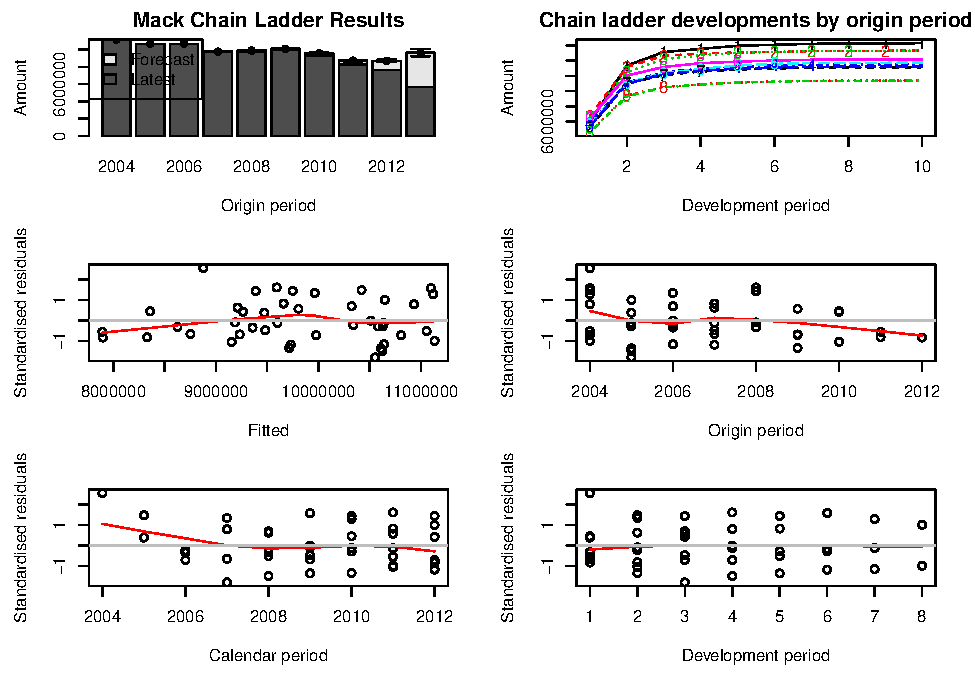
\includegraphics{LossDataAnalytics_files/figure-latex/ResidualPlot-1} \end{center}

The top left-hand plot is a bar-chart of the latest claims position plus
IBNR and Mack's standard error by occurrence period. The top right-hand
plot shows the forecasted development patterns for all occurrence
periods (starting with 1 for the oldest occurrence period).

When setting the argument \texttt{lattice=TRUE} we obtain a plot of the
development, including the prediction and estimated standard errors by
occurrence period:

\begin{Shaded}
\begin{Highlighting}[]
\KeywordTok{plot}\NormalTok{(CL, }\DataTypeTok{lattice=}\OtherTok{TRUE}\NormalTok{)}
\end{Highlighting}
\end{Shaded}

\begin{center}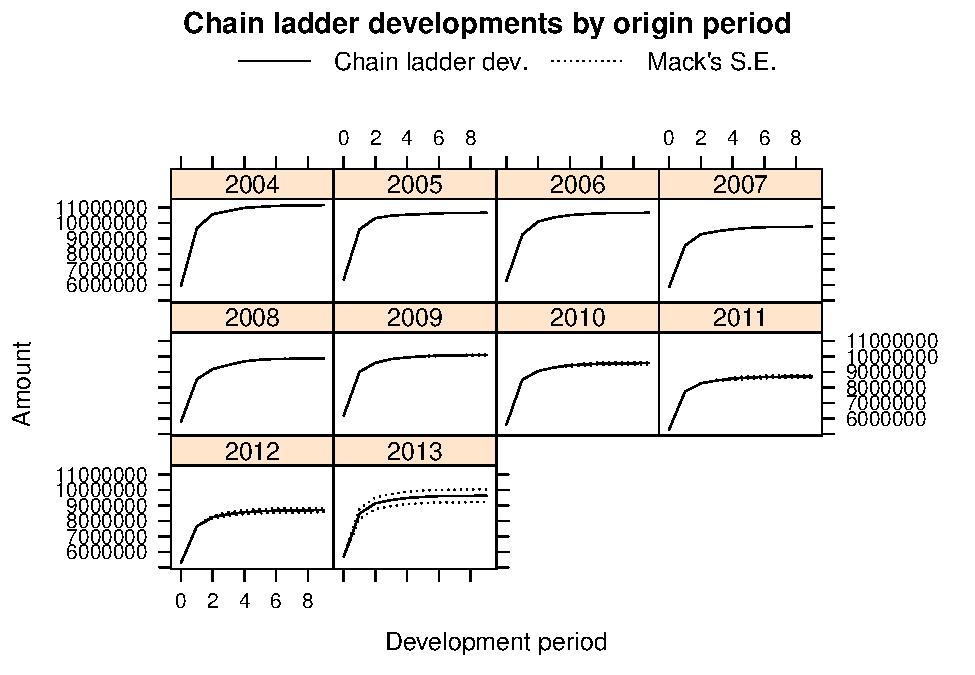
\includegraphics{LossDataAnalytics_files/figure-latex/PlotLattice-1} \end{center}

\section{GLMs and Bootstrap for Loss Reserves}\label{S:GLMs}

\begin{center}\rule{0.5\linewidth}{\linethickness}\end{center}

\textbf{This section is being written and is not yet complete nor
edited. It is here to give you a flavor of what will be in the final
version.}

\begin{center}\rule{0.5\linewidth}{\linethickness}\end{center}

This section covers regression models to analyze run-off triangles. When
analyzing the data in a run-off triangle with a regression model, the
standard toolbox for model building, estimation and prediction becomes
available. Using these tools we are able to go beyond the point estimate
and standard error as derived in Section \ref{S:Chain-ladder}. More
specifically, we build a generalized linear model (GLM) for the
incremental payments \(X_{ij}\) in Figure \ref{fig:tikz-triangle}.
Whereas the chain-ladder method works with cumulative data, typical GLMs
assume the response variables to be independent and therefore work with
incremental run-off triangles.

\subsection{Model Specification}\label{model-specification}

Let \(X_{ij}\) denote the incremental payment in cell \((i,j)\) of the
run-off triangle. We assume the \(X_{ij}\)s to be independent with a
density \(f(x_{ij};\theta_{ij},\phi)\) from the exponential family of
distributions. We identify

\begin{itemize}
\tightlist
\item
  \(\mu_{ij}=E[X_{ij}]\) the expected value of cell \(X_{ij}\)
\item
  \(\phi\) the dispersion parameter and
  \(\text{Var}[X_{ij}]=\phi \cdot V(\mu_{ij})\), where \(V(.)\) is the
  variance function
\item
  \(\eta_{ij}\) the linear predictor such that \(\eta_{ij}=g(\mu_{ij})\)
  with \(g\) the link function.
\end{itemize}

Distributions from the exponential family and their default link
functions are listed on
\url{http://stat.ethz.ch/R-manual/R-patched/library/stats/html/family.html}.
We now discuss three specific GLMs widely used for loss reserving.

First, the Poisson regression model was introduced in Section
\ref{S:RC:PoissonRegression}. In this model, we assume that \(X_{ij}\)
has a Poisson distribution with parameter

\[
\mu_{ij} = \pi_i \cdot \gamma_j,
\]

a cross-classified structure that captures a multiplicative effect of
the occurrence year \(i\) and the development period \(j\). The proposed
model structure is not identifiable without an additional constraint on
the parameters, e.g. \(\sum_{j=0}^J \gamma_j=1\). This constraint gives
an explicit interpretation to \(\pi_i\) (with \(i=1,\ldots,I\)) as the
exposure or volume measure for occurrence year \(i\) and \(\gamma_j\) as
the fraction of the total volume paid out with delay \(j\). However,
when calibrating GLMs in \texttt{R} alternative constraints such as
\(\pi_1=1\) or \(\gamma_1=1\), or a reparametrization where
\(\mu_{ij} = \exp{(\mu+\alpha_i+\beta_j)}\) are easier to implement. We
continue with the latter specification, including
\(\alpha_1 = \beta_0 = 0\), the so-called corner constraints. This GLM
treats the occurrence year and the payment delay as factor variables and
fits a parameter per level, next to an intercept \(\mu\). The corner
constraints put the effect of the first level of a factor variable equal
to zero. The Poisson assumption is particularly useful for a run-off
triangle with numbers of reported claims, often used in the estimation
of the number of IBNR claims (see Section \ref{S:Data}).

Second, an interesting modification of the basic Poisson regression
model is the \textbf{over-dispersed Poisson} regression model where
\(Z_{ij}\) has a Poisson distribution with parameter \(\mu_{ij}/\phi\)
and

\[
\begin{array}{rl}
X_{ij} &\sim  \phi \cdot Z_{ij}  \\
\mu_{ij} &= \exp{(\mu + \alpha_i + \beta_j)}.
\end{array}
\]

Consequently, \(X_{ij}\) has the same specification for the mean as in
the basic Poisson regression model, but now

\[
\text{Var}[X_{ij}] = \phi^2 \cdot \text{Var}[Z_{ij}] = \phi \cdot \exp{(\mu + \alpha_i + \beta_j)}.
\]

This construction allows for under (when \(\phi <1\)) and
over-dispersion (with \(\phi>1\)). Because \(X_{ij}\) no longer follows
a well-known distribution, this approach is referred to as
quasi-likelihood. It is particularly useful to model a run-off triangle
with incremental payments, as these typically reveal over-dispersion.

Third, the \textbf{gamma} regression model is relevant to model a
run-off triangle with claim payments. Recall from Section
\ref{S:Loss:Gamma} (see also the Appendix Chapter
\ref{C:SummaryDistributions}) with parameters \(\alpha\) and \(\theta\).
From these, we reparameterize and define a new parameter
\(\mu = \alpha \cdot \theta\) while retaining the scale parameter
\(\theta\). Further, assume that \(X_{ij}\) has a gamma distribution and
allow \(\mu\) to vary by \(ij\) such that

\[
\mu_{ij} =  \exp{(\mu + \alpha_i + \beta_j)}.
\]

\subsection{Model Estimation and
Prediction}\label{model-estimation-and-prediction}

We now estimate the regression parameters \(\mu\), \(\alpha_i\) and
\(\beta_j\) in the proposed GLMs. In \texttt{R} the \texttt{glm}
function is readily available to estimate these parameters via maximum
likelihood estimation (mle) or quasi-likelihood estimation (in the case
of the over-dispersed Poisson). Having the parameter estimates
\(\hat{\mu}\), \(\hat{\alpha}_i\) and \(\hat{\beta}_j\) available, a
point estimate for each cell in the upper triangle follows

\[
\hat{X}_{ij} =\hat{E[X_{ij}]} = \exp{(\hat{\mu}+\hat{\alpha}_i+\hat{\beta}_j)},\ \text{with}\ i+j\leq I.
\] Similarly, a cell in the lower triangle will be predicted as

\[
\hat{X}_{ij} = \hat{E[X_{ij}]} = \exp{(\hat{\mu}+\hat{\alpha}_i+\hat{\beta}_j)},\ \text{with}\ i+j> I.
\]

Point estimates for outstanding reserves (per occurrence year \(i\) or
the total reserve) then follow by summing the cell-specific estimates.
By combining the observations in the upper triangle with their point
estimates, we can construct properly defined residuals and use these for
residual inspection.

\subsection{Bootstrap}\label{bootstrap}

\section{Further Resources and
Contributors}\label{LossRe:further-reading-and-resources}

\subsubsection*{Contributors}\label{contributors-1}
\addcontentsline{toc}{subsubsection}{Contributors}

\begin{itemize}
\tightlist
\item
  \textbf{Katrien Antonio}, KU Leuven and University of Amsterdam,
  \textbf{Jan Beirlant}, KU Leuven, and \textbf{Tim Veerdonck},
  University of Antwerp, are the principal authors of the initial
  version of this chapter. Email:
  \href{mailto:katrien.antonio@kuleuven.be}{\nolinkurl{katrien.antonio@kuleuven.be}}
  for chapter comments and suggested improvements.
\end{itemize}

\subsubsection*{Further Readings and
References}\label{further-readings-and-references}
\addcontentsline{toc}{subsubsection}{Further Readings and References}

As displayed in Figure \ref{fig:tikz-run-off}, similar timelines and
visualizations are discussed (among others) in \citet{WuthrichMerz2008},
\citet{AntonioPlat2014} and \citet{WuthrichMerz2015}.

Over time actuaries started to think about possible underlying models
and we mention some important contributions:

\begin{itemize}
\tightlist
\item
  \citet{Kremer1982}: two-way ANOVA
\item
  \citet{Kremer1984}, \citet{Mack1991}: Poisson model
\item
  \citet{Mack1993}: distribution-free chain-ladder model
\item
  \citet{Renshaw1989}; \citet{RenshawVerrall1998}: over-dispersed
  Poisson model
\item
  \citet{Gisler2006}; \citet{GislerWuthrich2008}; \citet{Buhlmann2009}:
  Bayesian chain-ladder model.
\end{itemize}

The various stochastic models proposed in actuarial literature rely on
different assumptions and have different model properties, but have in
common that they provide exactly the chain-ladder reserve estimates. For
more information we also refer to \citet{MackVenter2000} and to the
lively discussion that was published in \emph{ASTIN Bulletin: Journal of
the International Actuarial Association} in 2006 \citep{Venter2006}.

To read more about exponential families and generalized linear models,
see, for example, \citet{McCullagh1989} and \citet{WuthrichMerz2008}. We
refer to \citep{Kremer1982}, \citep{RenshawVerrall1998} and
\citep{EnglandVerrall2002}, and the overviews in \citep{Taylor2000},
\citep{WuthrichMerz2008} and \citep{WuthrichMerz2015} for more details
on the discussed GLMs. XXX presents alternative distributional
assumptions and specifications of the linear predictor.

\bibliography{References/LDAReferenceC.bib,References/articles.bib,References/books.bib,References/packagesA.bib,References/packagesB.bib}


\end{document}
